%%%%%%%%%%%%%%%%%%%%%%%%%%%%%%%%%%%%%%%%%%%%%%%%%%%%%%%%%%%%%%%%%%%%%
%% This is a (brief) model paper using the achemso class
%% The document class accepts keyval options, which should include
%% the target journal and optionally the manuscript type. 
%%%%%%%%%%%%%%%%%%%%%%%%%%%%%%%%%%%%%%%%%%%%%%%%%%%%%%%%%%%%%%%%%%%%%
\documentclass[journal=jacsat,manuscript=article]{achemso}

%%%%%%%%%%%%%%%%%%%%%%%%%%%%%%%%%%%%%%%%%%%%%%%%%%%%%%%%%%%%%%%%%%%%%
%% Place any additional packages needed here.  Only include packages
%% which are essential, to avoid problems later. Do NOT use any
%% packages which require e-TeX (for example etoolbox): the e-TeX
%% extensions are not currently available on the ACS conversion
%% servers.
%%%%%%%%%%%%%%%%%%%%%%%%%%%%%%%%%%%%%%%%%%%%%%%%%%%%%%%%%%%%%%%%%%%%%
\usepackage[version=3]{mhchem} % Formula subscripts using \ce{}
\usepackage{natbib}

%\usepackage{epsfig,amsfonts,amsmath,graphicx,dcolumn,bm,amssymb,authblk,cite,epstopdf,times,fullpage,placeins}
%\usepackage{float}
%\usepackage{lettrine}
%\usepackage{cuted}
%\usepackage{soul}
%\usepackage[usenames, dvipsnames]{color}
%\usepackage[hmargin=2.5cm,vmargin=3cm]{geometry}
%\usepackage{xcolor}

%%%%%%%%%%%%%%%%%%%%%%%%%%%%%%%%%%%%%%%%%%%%%%%%%%%%%%%%%%%%%%%%%%%%%
%% If issues arise when submitting your manuscript, you may want to
%% un-comment the next line.  This provides information on the
%% version of every file you have used.
%%%%%%%%%%%%%%%%%%%%%%%%%%%%%%%%%%%%%%%%%%%%%%%%%%%%%%%%%%%%%%%%%%%%%
%%\listfiles

%%%%%%%%%%%%%%%%%%%%%%%%%%%%%%%%%%%%%%%%%%%%%%%%%%%%%%%%%%%%%%%%%%%%%
%% Place any additional macros here.  Please use \newcommand* where
%% possible, and avoid layout-changing macros (which are not used
%% when typesetting).
%%%%%%%%%%%%%%%%%%%%%%%%%%%%%%%%%%%%%%%%%%%%%%%%%%%%%%%%%%%%%%%%%%%%%
\newcommand*\mycommand[1]{\texttt{\emph{#1}}}

%%%%%%%%%%%%%%%%%%%%%%%%%%%%%%%%%%%%%%%%%%%%%%%%%%%%%%%%%%%%%%%%%%%%%
%% Meta-data block
%% ---------------
%% Each author should be given as a separate \author command.
%%
%% Corresponding authors should have an e-mail given after the author
%% name as an \email command. Phone and fax numbers can be given
%% using \phone and \fax, respectively; this information is optional.
%%
%% The affiliation of authors is given after the authors; each
%% \affiliation command applies to all preceding authors not already
%% assigned an affiliation.
%%
%% The affiliation takes an option argument for the short name.  This
%% will typically be something like "University of Somewhere".
%%
%% The \altaffiliation macro should be used for new address, etc.
%% On the other hand, \alsoaffiliation is used on a per author basis
%% when authors are associated with multiple institutions.
%%%%%%%%%%%%%%%%%%%%%%%%%%%%%%%%%%%%%%%%%%%%%%%%%%%%%%%%%%%%%%%%%%%%%
\author{Gabriel Guendelman}
\affiliation[First University]
{AMOS and Department of Chemical and Biological Physics, Weizmann Institute of Science, 76100 Rehovot, Israel}
\email{gabriel.guendelman@weizmann.ac.il}
\phone{+972 (0)8 9343673}
%\fax{+123 (0)123 4445557}
\author{Yulia Lovsky}
\affiliation[First University]
{AMOS and Department of Chemical and Biological Physics, Weizmann Institute of Science, 76100 Rehovot, Israel}
\author{Eyal Yakobi}
\affiliation[Second University]
{Soreq NRC, Yavne, Israel}
\author{Ori Mor}
\affiliation[First University]
{AMOS and Department of Chemical and Biological Physics, Weizmann Institute of Science, 76100 Rehovot, Israel}
\author{Ifat Kaplan-Ashiri}
\affiliation[Third University]
{Department of Chemical Research Support, Weizmann Institute of Science, 76100 Rehovot, Israel}
\author{Ohad Goldbart}
\affiliation[Fourth University]
{Department of Materials and Interfaces, Weizmann Institute of Science,  76100  Rehovot,  Israel}
\author{Barak Dayan}
\affiliation[First University]
{AMOS and Department of Chemical and Biological Physics, Weizmann Institute of Science, 76100 Rehovot, Israel}
\email{barak.dayan@weizmann.ac.il}

%%%%%%%%%%%%%%%%%%%%%%%%%%%%%%%%%%%%%%%%%%%%%%%%%%%%%%%%%%%%%%%%%%%%%
%% The document title should be given as usual. Some journals require
%% a running title from the author: this should be supplied as an
%% optional argument to \title.
%%%%%%%%%%%%%%%%%%%%%%%%%%%%%%%%%%%%%%%%%%%%%%%%%%%%%%%%%%%%%%%%%%%%%
\title[An \textsf{achemso} demo]
  {Sensing of arbitrarily shaped nanoparticles by Whispering Gallery Mode resonators}

%%%%%%%%%%%%%%%%%%%%%%%%%%%%%%%%%%%%%%%%%%%%%%%%%%%%%%%%%%%%%%%%%%%%%
%% Some journals require a list of abbreviations or keywords to be
%% supplied. These should be set up here, and will be printed after
%% the title and author information, if needed.
%%%%%%%%%%%%%%%%%%%%%%%%%%%%%%%%%%%%%%%%%%%%%%%%%%%%%%%%%%%%%%%%%%%%%
\abbreviations{IR,NMR,UV}
\keywords{American Chemical Society, \LaTeX}

%%%%%%%%%%%%%%%%%%%%%%%%%%%%%%%%%%%%%%%%%%%%%%%%%%%%%%%%%%%%%%%%%%%%%
%% The manuscript does not need to include \maketitle, which is
%% executed automatically.
%%%%%%%%%%%%%%%%%%%%%%%%%%%%%%%%%%%%%%%%%%%%%%%%%%%%%%%%%%%%%%%%%%%%%
\begin{document}

%%%%%%%%%%%%%%%%%%%%%%%%%%%%%%%%%%%%%%%%%%%%%%%%%%%%%%%%%%%%%%%%%%%%%
%% The "tocentry" environment can be used to create an entry for the
%% graphical table of contents. It is given here as some journals
%% require that it is printed as part of the abstract page. It will
%% be automatically moved as appropriate.
%%%%%%%%%%%%%%%%%%%%%%%%%%%%%%%%%%%%%%%%%%%%%%%%%%%%%%%%%%%%%%%%%%%%%
\begin{tocentry}

Some journals require a graphical entry for the Table of Contents.
This should be laid out ``print ready'' so that the sizing of the
text is correct.

Inside the \texttt{tocentry} environment, the font used is Helvetica
8\,pt, as required by \emph{Journal of the American Chemical
Society}.

The surrounding frame is 9\,cm by 3.5\,cm, which is the maximum
permitted for  \emph{Journal of the American Chemical Society}
graphical table of content entries. The box will not resize if the
content is too big: instead it will overflow the edge of the box.

This box and the associated title will always be printed on a
separate page at the end of the document.

\end{tocentry}

%%%%%%%%%%%%%%%%%%%%%%%%%%%%%%%%%%%%%%%%%%%%%%%%%%%%%%%%%%%%%%%%%%%%%
%% The abstract environment will automatically gobble the contents
%% if an abstract is not used by the target journal.
%%%%%%%%%%%%%%%%%%%%%%%%%%%%%%%%%%%%%%%%%%%%%%%%%%%%%%%%%%%%%%%%%%%%%
\begin{abstract}
Whispering gallery mode (WGM) microresonators are a promising platform for highly sensitive, label-free detection and probing of individual nano-objects. The high Purcell factor of state of the art WGM microresonators allows strong interactions between photons and nano-particles, molecules or even single atoms positioned within the evanescent field of the microresonator. Variations in the measured spectrum can be attributed to the optical and structural properties of the nano-object.

So far, most of the works focused on the detection and sizing of spherical nano-objects. Our work focuses on 3-D characterization of arbitrary shaped nanoparticles.  We introduce and experimentally implement a new theoretical model that comprehensively describes interactions between arbitrarily shaped nanoparticles with arbitrarily polarized WGM, taking into account a set of effects that are often not considered or neglected. These effects include the elliptical, often close to circular, polarization of the transverse magnetic (TM) mode, the possible non-spherical shape of the nanoparticle and its finite size, and the lossy, ‘open-system’ nature of the normal optical modes. We also introduce a self-referencing measurement method that allows the extraction of information from measurements done at arbitrary positions within the WGM. We verify this model by experimentally scanning the position and orientation of a single \ce{WS_2} nanotube within the evanescent region of a WGM of a silica microtoroid resonator inside a scanning electron-microscope (SEM). Using our model we perform 3-D characterization of the nanotube, namely extract the ratios between the real and imaginary parts of its polarizability along both axes.

Our model allows harnessing the ultrahigh sensitivity of detection using the WGM to extract rich and accurate 3-D information on the structure of various nano-objects and other important properties such as chirality and conformational changes.
\end{abstract}

%%%%%%%%%%%%%%%%%%%%%%%%%%%%%%%%%%%%%%%%%%%%%%%%%%%%%%%%%%%%%%%%%%%%%
%% Start the main part of the manuscript here.
%%%%%%%%%%%%%%%%%%%%%%%%%%%%%%%%%%%%%%%%%%%%%%%%%%%%%%%%%%%%%%%%%%%%%
\section{Introduction}
Optical microresonators are at the heart of a wide range of applications and studies~\cite{vahala2003optical}. Particularly, WGM microcavities such as microspheres~\cite{arnold2003shift,vernooy1998high}, microdisks~\cite{savchenkov2004kilohertz}, microbottles~\cite{louyer2005tunable} and microtoroids~\cite{armani2003} resonantly confine light to small volumes and can serve as highly sensitive label-free detectors~\cite{vollmer2008whispering,vollmer2012}. Single-particle detection and sizing of spherical nano-objects using WGM cavities was successfully implemented~\cite{vollmer2008single,zhu2010,lu2011,dantham2012}, yet so far sensing of non-spherical particles has been limited to monolayers~\cite{noto2007,topolancik2007photoinduced} or large nano-objects~\cite{ren2007highQ,kim2012detection}. The characterization of non-spherical particles was performed by measuring the shifts of a single Lorentzian dip resonance of the microresonator ~\cite{arnold2003shift}. This method was applied later to characterize a layer of uniaxial particles by measuring the spectral changes of the TE and the TM modes. Here we suggest an approach for 3D characterization of arbitrarily shape nanoparticle based on measuring the splitting of a single Lorentzian resonance. Mode splitting arises when two counterpropagating modes, ideally degenerated, are spectrally split due to perturbations in the surface or the surrounding of the microcavity. This might be caused by a nanoparticle entering the optical mode of the microcavity; the spectral properties of the mode splitting can be then correlated to the optical properties of a nanoparticle.
While there are numerical simulations that include the complete polarization structure of TE and TM modes and can be applied to non-spherical particles (e.g. a finite element COMSOL simulation~\cite{kaplan2013finite}), there is a need in a comprehensive analytical model that can connect between the three-dimensional properties of the interacting nanoparticle to the observed WGM spectrum.

In this work, we suggest such a model and characterize a single \ce{WS_2} nanotube using a high-Q toroidal microresonator by independently probing the whispering gallery TE and TM modes along the equator. We then correlate the induced spectral changes to the optical properties of the nanotube.

The analytical model we developed is an extension for non-spherical particles of the formalism introduced by Mazzei \latin{et al.}~\cite{mazzei2007}, which was later generalized to treat more than one scatterer~\cite{yi2011multiple} .

The model gives the full description of how the spectral changes (of both TE and TM) depend on the coupling and loss rates, and how these rates depend on the linear (TE) or elliptical (TM)~\cite{junge2013strong,axelrod1984total,kawalec2007spectroscopic} polarization of the optical mode and the polarizability properties of arbitrarily shaped nanoparticle, which allows the 3D characterization. The model takes into account the asymmetric backscattering between the counterpropagating modes that arise when the losses of the system are significant~\cite{wiersig2011structure,peng2016chiral,zhu2010contorolled}. It also takes into account the effect of the imaginary part of the polarizability tensor~\cite{hu2014mode} and the finite size of the nanoparticle on the induced spectral changes. Also, to overcome the strong effect of the exact position of the nanoparticle on the measurement we propose a self-referenced method of measurement that allows real-time monitoring of the particle position in the standing wave pattern.

\section{The analytical model}

\subsection{Cavity model}

WGM resonators support two counterpropagating modes (see Fig.~\ref{fig:torusTMTE}). Ideally, these two modes are degenerate; however surface roughness and other defects couple between the counterpropagating modes, lifting this degeneracy. Such a system is described by the normal modes, which appear as the split mode spectrum~\cite{Haroche1995splitting,Kippenberg:02,zhu2010,kim2010}.
\begin{figure}[H]
\centering
             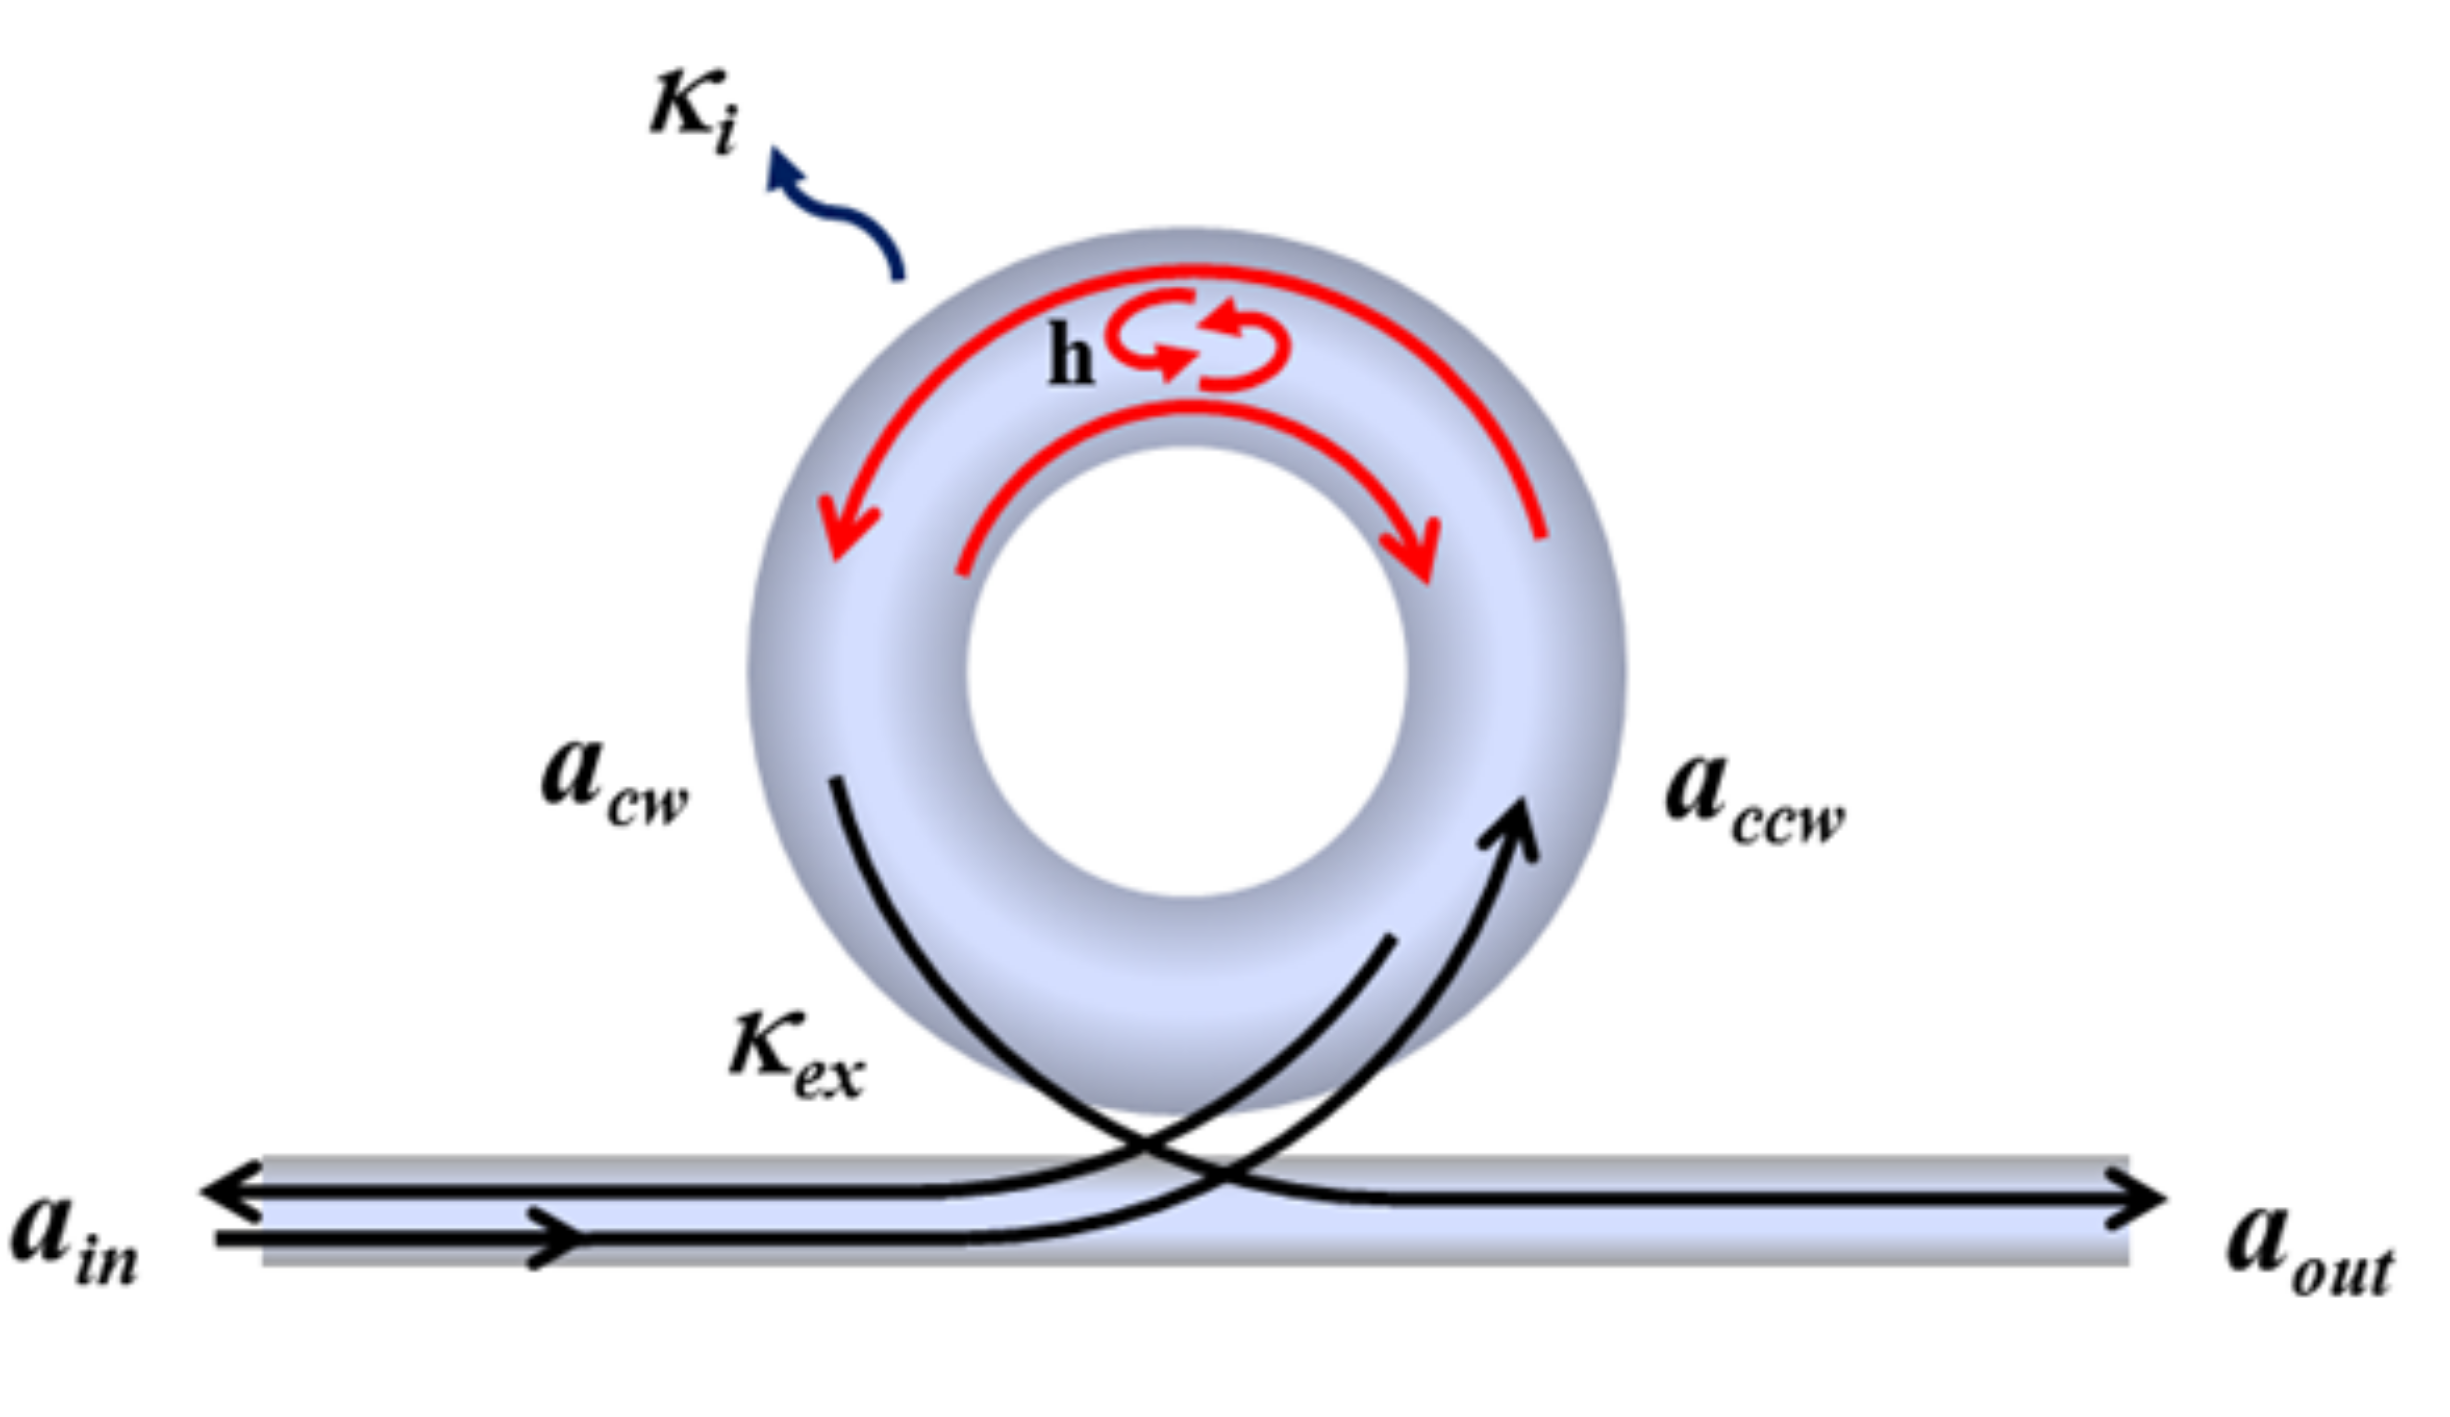
\includegraphics[trim=0cm 1.0cm 0.5cm 0.5cm, clip, width=0.5\textwidth]{Images/cw_ccw.png}
             \caption{\textbf{Bare cavity model sketch.} Illustration of the fiber-coupled WGM resonator where light is sent from one direction, its modes ($a_{in}, a_{out}, a_{cw}, a_{ccw}$), and corresponding rates ($\kappa_i, \kappa_{ex}, h$). 
              \label{fig:torusTMTE}}
  \end{figure}
The expressions for the two eigenvalues of the normal modes, either of the TE or the TM mode, of a bare cavity are~\cite{mazzei2007}: $\displaystyle \omega_{\pm}=\omega_c \pm h - i \kappa$, where $\omega_c$ is the resonance central frequency, $\kappa$ is the total loss rate of a bare cavity, and $\textit{h}$ is the intrinsic coupling rate between the clockwise (\textit{cw}) and the counterclockwise (\textit{ccw}) propagating modes due to surface roughness.

When a nanoparticle is positioned in the optical mode it can absorb or scatter light. The scattered light can couple coherently back into the same mode or backscatter into the counterpropagating mode, or be lost incoherently scattering to the free-space modes. The backscattering causes an additional coupling between the counterpropagating modes, hence causes an additional splitting of the spectrum. Scattering into the same mode causes a total shift of both normal modes. Loss due to scattering or absorption causes broadening of the normal modes spectrum.

To find the new complex eigenfrequencies of the cavity we need to solve a new set of equations of motion. We write the non-Hermitian Hamiltonian \textbf{[add ref - Nimrod?]} for the counter-propagating modes, which includes coupling and loss due to the nanoparticle, in the following way:
\begin{equation}
\mathcal{H} = \mathcal{H}_{cavity} + \mathcal{H}_{coupling} + \mathcal{H}_{loss}
\end{equation}
where $\mathcal{H}_{cavity}$ describes the uncoupled cavity modes without intrinsic scattering:
\begin{equation}
\mathcal{H}_{cavity} = \sum_{k=cw,ccw} \hbar \omega_c a_{k}^{\dagger} a_{k} 
\end{equation}
$a_{k}$ and $a_{k}^{\dagger}$ are the annihilation and creation operators, respectively, in mode $k$. $\mathcal{H}_{coupling}$ describes the coupling between the counterpropagating modes:
\begin{equation}
\begin{split}
\mathcal{H}_{coupling} = &\hbar h \left( a_{cw}^{\dagger} a_{ccw} + a_{ccw}^{\dagger} a_{cw} \right) \\
&- i \frac{\hbar}{2} \sum_{k,k'=cw,ccw} \left( g_{k,k'} a_{k}^{\dagger} a_{k'} + h.c. \right)
\end{split}
\end{equation}
where $g_{k,k'}$ is the complex coupling rate between two propagating modes, which is induced by the part of the particle polarizability in the optical mode. $\mathcal{H}_{loss}$ describes the cavity losses due to scattering and absorption:
\begin{equation}
\begin{split}
\mathcal{H}_{loss} = &- i \hbar \sum_{k,k'=cw,ccw} \left( \gamma_{s,k,k'} + \gamma_{a,k,k'} \right) a_{k}^{\dagger} a_{k'} \\
&- i \hbar \sum_{k=cw,ccw} \kappa_i a_{k}^{\dagger} a_{k}
\end{split}
\end{equation}
The first term of $\mathcal{H}_{loss}$ describes the losses, scattering ($\gamma_s$) and absorption ($\gamma_a$), due to presence of the particle. The second term represents the intrinsic cavity loss ($\kappa_i$).

From the given Hamiltonian one can derive the following set of coupled linear equations of motion:
\begin{equation}
\begin{split}
\omega a_{cw} &= C a_{cw} + D_1 a_{ccw} \\
\omega a_{ccw} &= C a_{ccw} + D_2 a_{cw}
\end{split}
\end{equation}
where,
\begin{equation}
\begin{split}
C &= \omega_c + g_{ccw,ccw} -i \left(\kappa_t + \gamma_{s,ccw,ccw} + \gamma_{a,ccw,ccw}\right) \\
  &= \omega_c + g_{cw,cw} -i \left( \kappa_t + \gamma_{s,cw,cw} + \gamma_{a,cw,cw} \right) \\
D_1 &= g_{cw,ccw} + h - i \left(\gamma_{s,cw,ccw} + \gamma_{a,cw,ccw} \right) \\
D_2 &= g_{ccw,cw} + h - i \left(\gamma_{s,ccw,cw} + \gamma_{a,ccw,cw} \right)
\end{split}
\end{equation}
The subscripts of coupling and loss rates specify the modes that are involved in the interaction. Mathematically, they have a different phase dependance: $\left\{g, \gamma_s, \gamma_a \right\}_{k,k'} \propto e^{- i \left(\beta_k - \beta_{k'} \right) x}$~\cite{yi2011multiple}.
Solving the equations of motion gives the new complex eigenfrequencies, $\omega_{\pm}$ of the form:
\begin{equation}
\omega_{\pm} = C \pm \sqrt{D_1 D_2}
\end{equation}
The real parts of $\omega_{\pm}$ are the center frequencies of the two normal modes. The imaginary parts correspond to the widths of the normal mode resonances by $\Gamma_{\pm} = 2 Im\left\{ \omega_{\pm} \right\}$.

The normal modes shifts and broadening changes are obtained by taking the difference between the new eigenmodes and the bare cavity normal modes. We denote the shifts (broadening changes) of the symmetric and antisymmetric normal modes by $\delta \omega_+$ ($\delta \Gamma_+$) and $\delta \omega_-$ ($\delta \Gamma_-$), respectively:
\begin{equation}
\begin{split}
\delta \omega_{\pm} &= Re \left\{ \omega_{\pm} \right\} - \omega_c \mp h \\
\delta \Gamma_{\pm} &= Im \left\{ \omega_{\pm} \right\} + \kappa_t
\end{split}
\label{eq:splitting_broadening}
\end{equation}
In split mode sensing it is convenient to use the difference between spectral changes, the splitting~\cite{zhu2010} $2 \Delta \omega$ and the difference between the broadenings~\cite{shao2013detection} $2 \Delta \Gamma$ of the normal modes.
\begin{equation}
\begin{split}
\Delta \omega_{\pm} &= \frac{1}{2} \left( \omega_{-} - \omega_{+} \right)\\
\Delta \Gamma_{\pm} &= \frac{1}{2} \left( \Gamma_{-} - \Gamma_{+} \right)
\end{split}
\end{equation}
We find it convenient to define also the average shift and the average broadening:
\begin{equation}
\begin{split}
S \omega_{\pm} &= \frac{1}{2} \left( \omega_{-} + \omega_{+} \right)\\
S \Gamma_{\pm} &= \frac{1}{2} \left( \Gamma_{-} + \Gamma_{+} \right)
\end{split}
\end{equation}
In particular, we normalize half the splitting and half the broadening difference by the average shift and average broadening, respectively. This eliminates the dependence on the mode properties, such as mode volume or the position of the particle in the mode, to allow accurate measurement of the nanoparticle properties.

\subsection{Cavity particle interaction}

The induced coupling rate and losses depend on the material properties and shape of the nanoparitcle, given by the polarizability tensor, $\bar{ \bar\alpha}$, and on the orientation of the (non spherical) particle in the optical field. We use the dipole approximation \textbf{[add refs]}, that dictates a linear relation between the applied external electric field $ \vec {\mathcal {E}}$ and the induced polarization $\vec P$ in the particle: $ \vec {P} =\mathcal{R}e [\bar{ \bar \alpha}] \vec {\mathcal E} $. Accordingly, the coupling energy between the counterpropagating modes, given by the perturbation energy $ \vec {P} \cdot \vec {\mathcal E}^*$ caused by the particle is:
\begin{equation}\label{g_k_ktag}
    \hbar g_{k,k'}=  - \mathcal{R}e [\bar{\bar \alpha}] ~\vec{ \mathcal{E}}_k \cdot  \vec{ \mathcal{E}}^*_{k'}
\end{equation}
The expression of the induced coupling rate between the counterpropagating modes of the TE linearly polarized field by a spherical particle was given by \textbf{[add refs]}:
\begin{equation} \label{eq:g_TE_nanotube}
g^{TE}_{k,k'} = - g e^{\pm i \Delta\beta x}
\end{equation}
where we wrote explicitly the azimuthal dependence of the WGM ($e^{im\phi}=e^{-i\beta_k x}$) along the equator of the mictroresonator, with $2\beta x $ in the exponent being the phase difference between the two counterpropagating modes and the $\pm$ sign corresponds to the \textit{ccw} $\rightarrow$ \textit{cw} and \textit{cw} $\rightarrow$ \textit{ccw} directions of coupling.
The expression for interaction with a circularly polarized field is of the form,
\begin{equation} \label{eq:g_TM_nanotube}
    g^{TM}_{k,k'} = - \left ( g \pm ig_{cp} \right) e^{\pm i \Delta\beta x}
\end{equation}
where we define two in-quadrature terms, in accordance with the two in-quadrature components of the TM electrical field.

The loss rate is the sum of the absorption loss rate $\gamma_a$, which is proportional to the imaginary part of the polarizability tensor $\mathcal{I}m[\bar{ \bar \alpha}]$ and the scattering loss rate $\gamma_s$, which is proportional to $|\alpha|^2$. The loss rate is also dependent on the polarization of the field and the orientation of the particle relative to it.
\begin{figure}[H]
\centering
             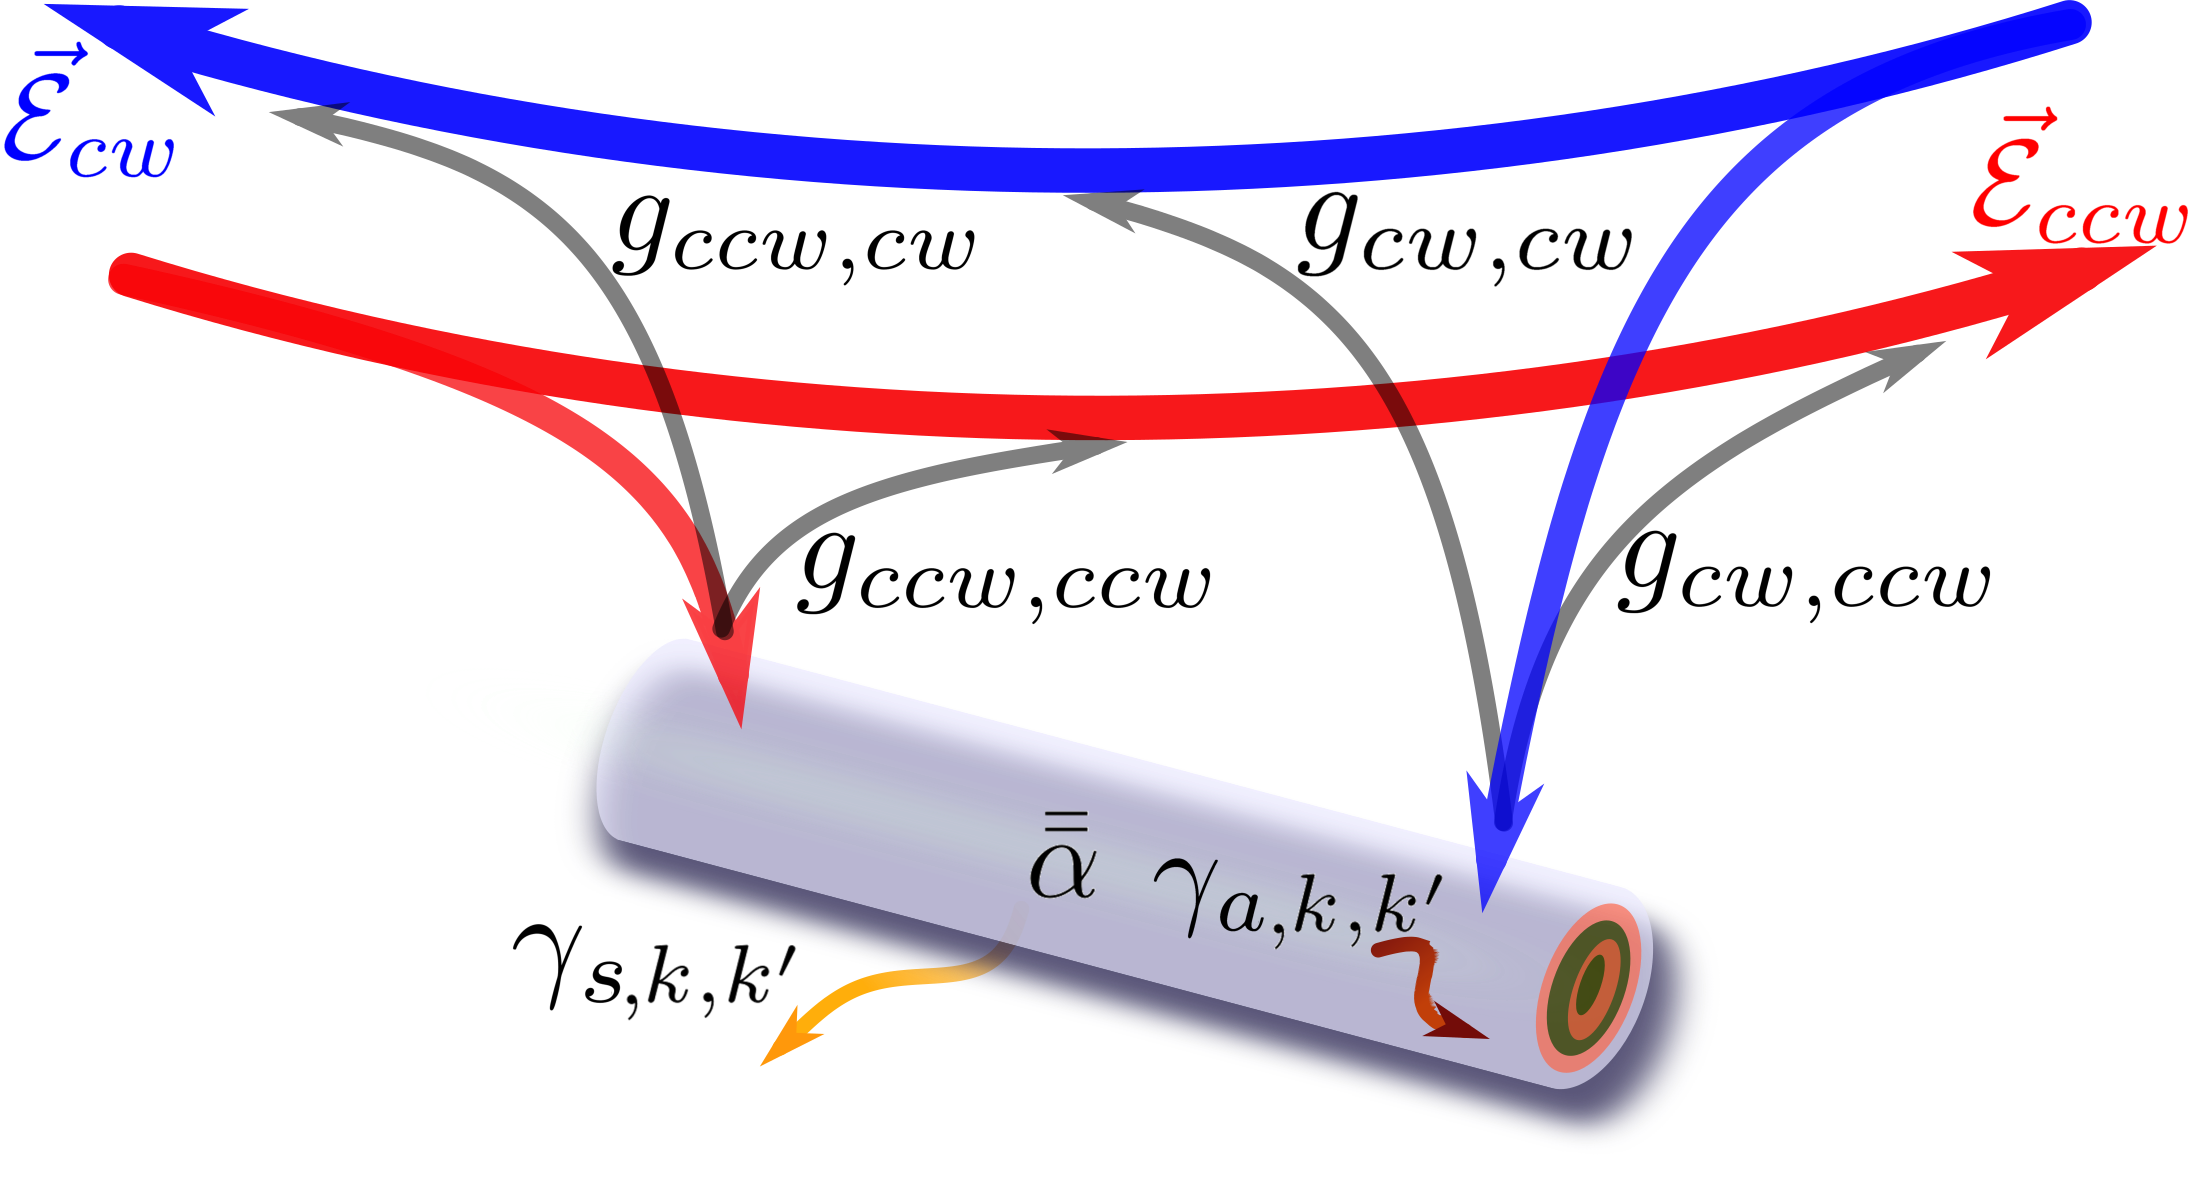
\includegraphics[trim=0cm 0.0cm 0.0cm 0.0cm, clip, width=0.5\textwidth]{Images/interaction.png}
             \caption{\textbf{Rates of interaction.} }
              \label{fig:cavity_tube_int}
  \end{figure}\vspace{-1cm}

\section{Methods}

\subsection{Calculation: sensing of a spherical particle with different WGM polarizations}

The induced spectral shifts and broadening strongly depend on the polarization of the mode.  Fig.~\ref{fig:TETMcompare} we illustrate the sensitivity of linearly polarized TE modes as well as circular and elliptical polarization of the TM mode to the presence of a spherical particle. For example, Fig.~\ref{fig:TETMcompare}e shows that the splitting signal of a perfect circularly polarized TM mode is insensitive to spherical particles at all (the red and the black curves that represent the shift of the symmetric and antisymmetric normal modes, respectively, coincide). This is because coherently scattered light from a polarization-preserving spherical particle cannot couple light into the orthogonally polarized mode and induce splitting, therefore both normal modes are red-shifted together (and have the same broadening). Detection of spherical particles using a perfectly circularly polarized TM mode is still possible by measuring the average shift (or average broadening) of the normal modes.

In Fig.~\ref{fig:TETMcompare}c we show the case of elliptically polarized TM mode, such as in silica WGM microresonators in air or water (see Supplementary Material). The counterpropagating elliptically polarized fields give rise to a slightly intensity-modulated pattern due to the particle presence (Fig.~\ref{fig:TETMcompare}f). This means that a splitting signal of a typical TM mode could indeed be used even for the sensing of spherical nanoparticles, although showing lower signal compared to the linearly polarized TE mode (Fig.~\ref{fig:TETMcompare}d). For example, for a silica microresonator in air, the maximum induced change in the splitting of the TM mode is only $\approx 34\%$ of the induced change in splitting of the TE mode (for a silica microresonator in water it is $\approx 70 \%$).

\begin{figure}[H]
\centering
                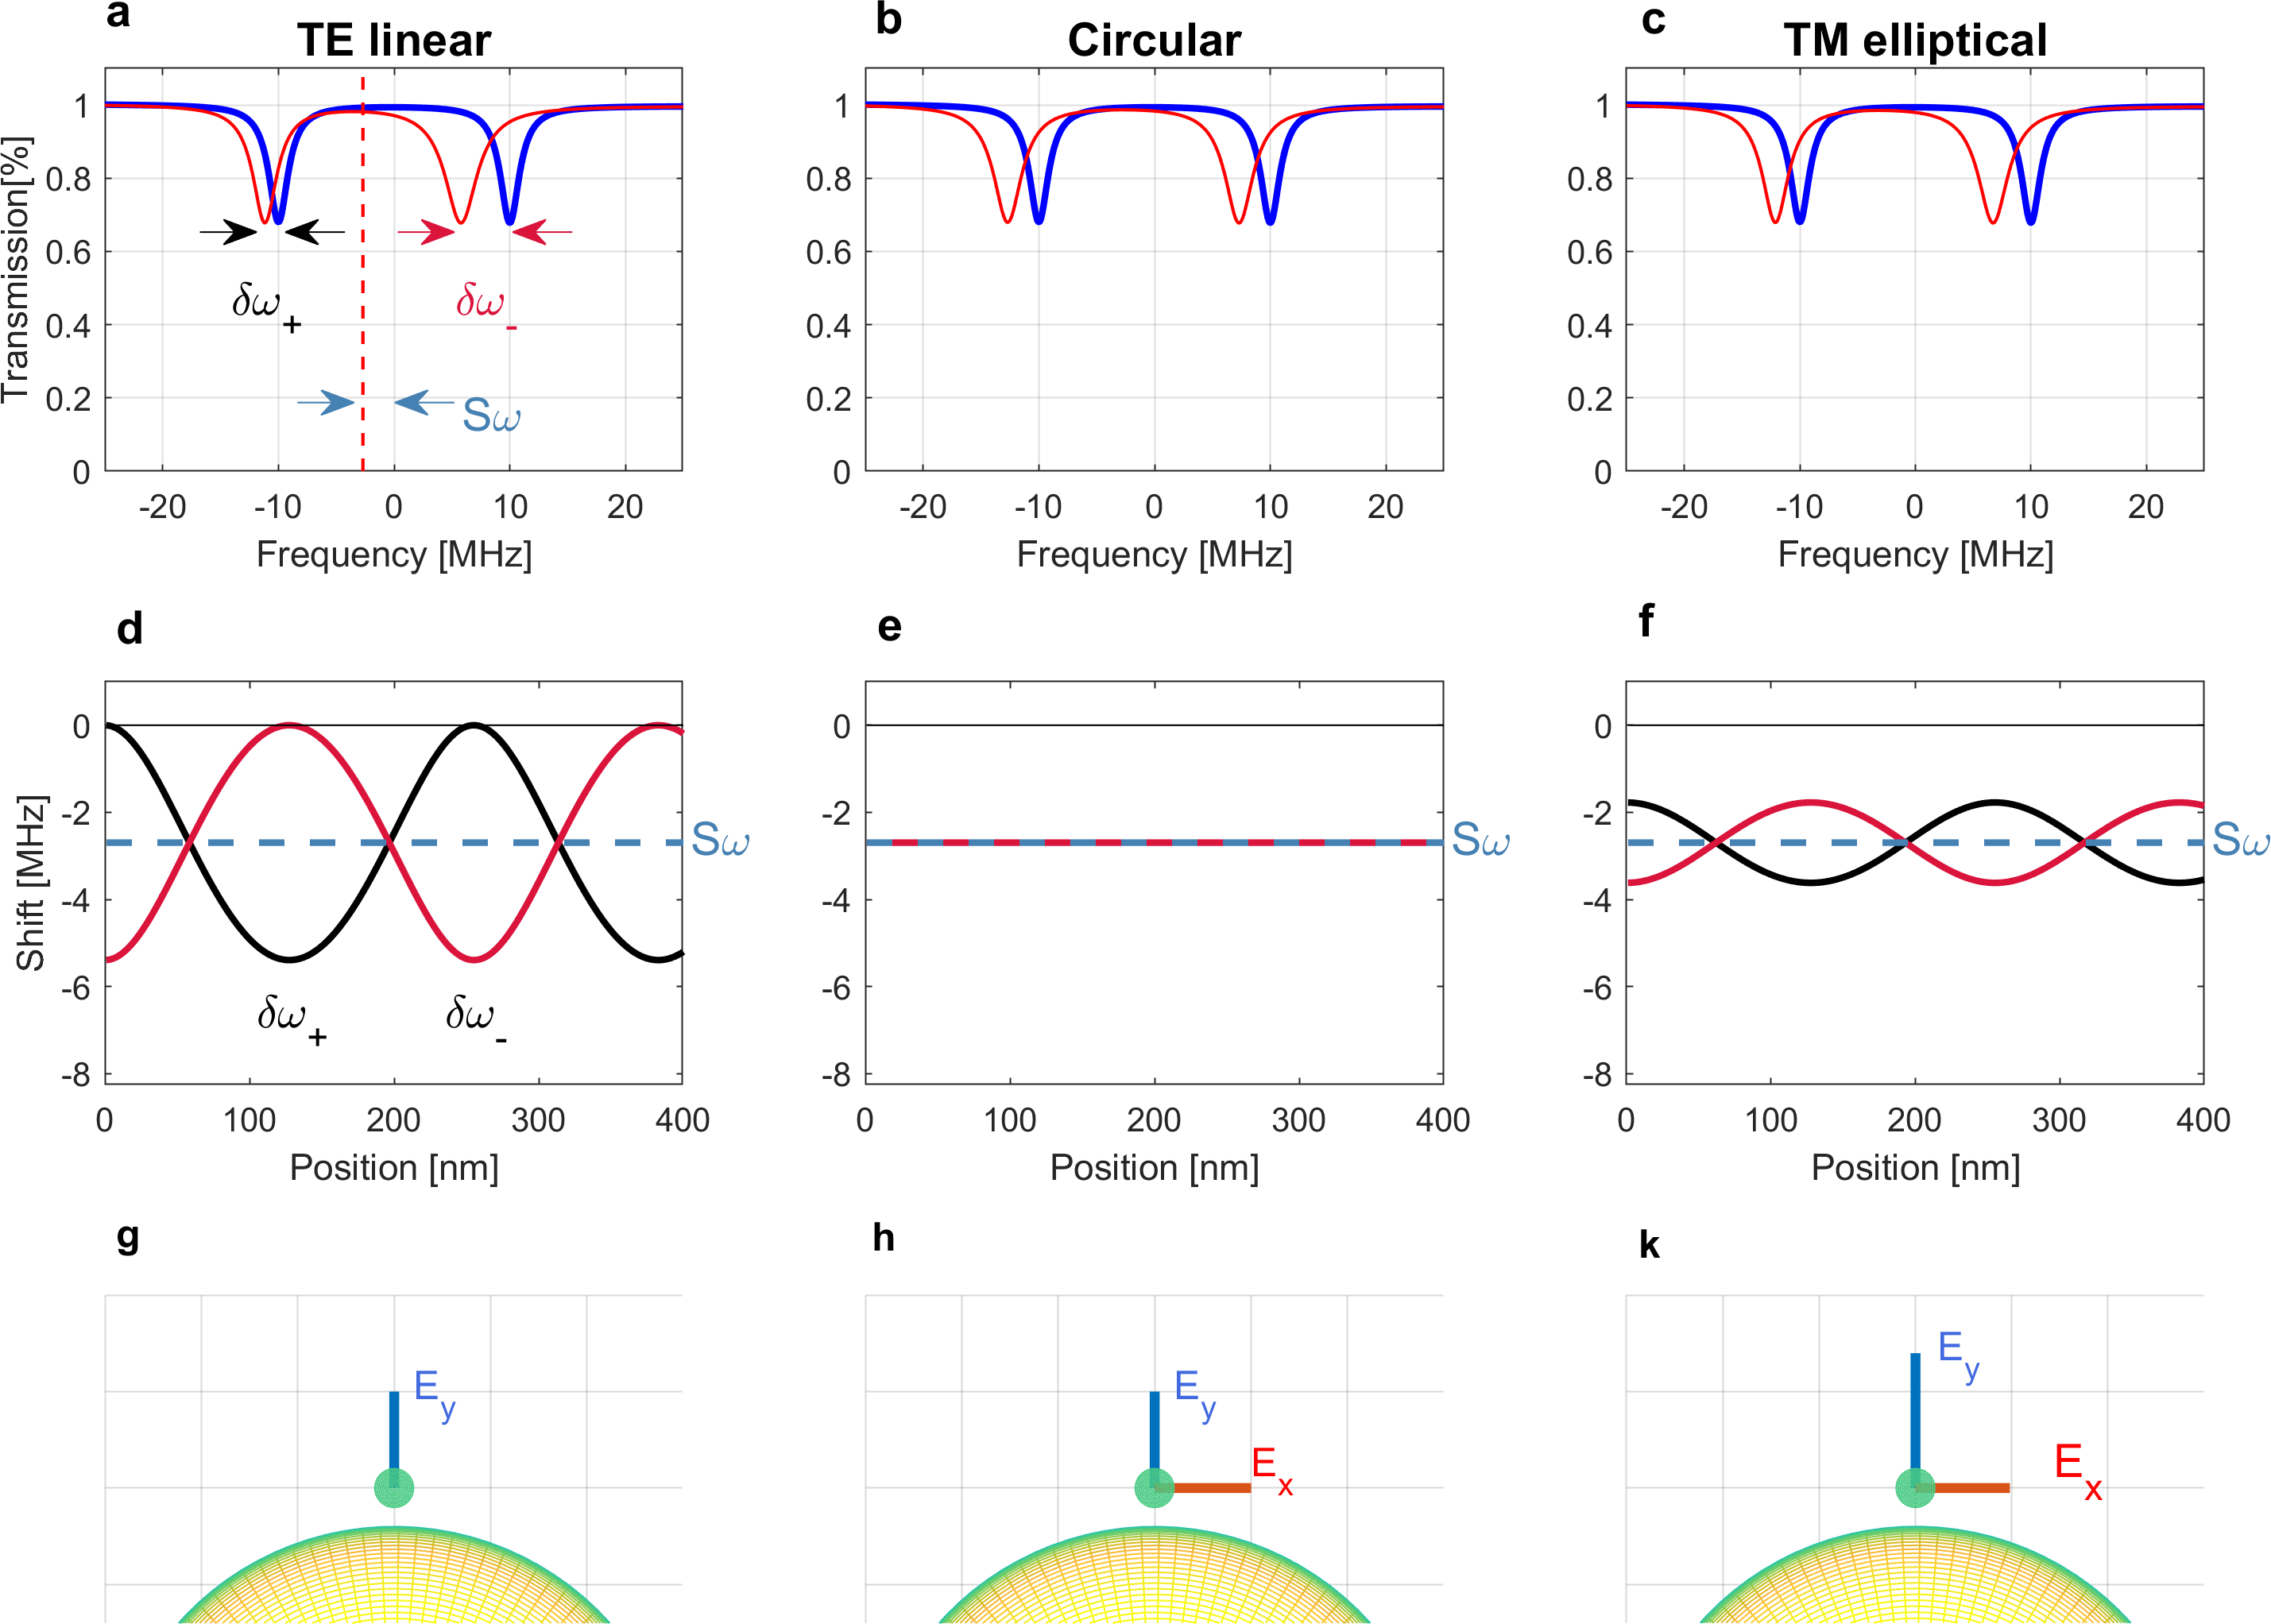
\includegraphics[trim=0.0cm 0.0cm 0.0cm 0.0cm, clip, width=0.95\textwidth]{Images/TMspherical_modified_3.png}\quad
             \caption{\textbf{Sensing of a spherical dielectric particle using the TM mode.} \textbf{a-c,} The spectral changes upon introduction of a spherical, $120nm$ in diameter, polystyrene nanoparticle inside the optical mode (for details see methods). The bare cavity spectrum (blue curve) is changed due to the presence of the particle (red curve) inside a linearly polarized mode (a). The induced spectral changes of a perfectly circularly polarized TM mode (b) and of typical TM mode with an elliptical polarization (c). (d)-(f) show the shifts ($\delta \omega$) of the symmetric (red curves) and antisymmetric (black curves) normal modes as a function of the position of the particle on the equator (eq.~\ref{eq:splitting_broadening}) of the linearly (d), circularly (e) and elliptically (f) polarized TM vs. the position of the nanoparticle along the equator.  The induced splitting signal is given by subtraction between the red and the black curves in (d)-(f) (not shown). The average shift is shown with the dash blue lines and marked by \textit{S}$\omega$.
						\label{fig:TETMcompare}}
\end{figure}

\subsection{Experiment: Optical characterization of a single WS2 nanotube and model verification}

A $\ce{WS_2}$ nanotube with an outer diameter of $60nm$ is brought close to the surface of a silica microtoroid and placed at the equatorial level, perpendicularly to the surface with nanometer accuracy. This was possible by conducting the experiment in a customized SEM vacuum chamber (Fig. \ref{fig:experiment}a).
While monitoring the exact position of the nanotube using the SEM, we measure the induced spectral shifts and broadening of the TE and TM polarized normal modes. These are then correlated to the polarizability tensor of the particle or its orientation.

An example of a single shot spectra with the nanotube brought into the evanescent field of a microtoroidal WGM resonator is shown the red and blue curves in Fig. \ref{fig:experiment}c, respectively. Fig. \ref{fig:experiment}d shows the shift of the symmetric and asymmetric modes and the induced splitting (the difference between the shifts) at one, arbitrarily chosen, along the equator, recorded over time. The modulation of the nanotube position near the surface allows a repeatable measurement with and without the perturbation and an accurate estimation of the induced shifts and broadening of the normal modes.

\begin{figure}[H]
\centering
          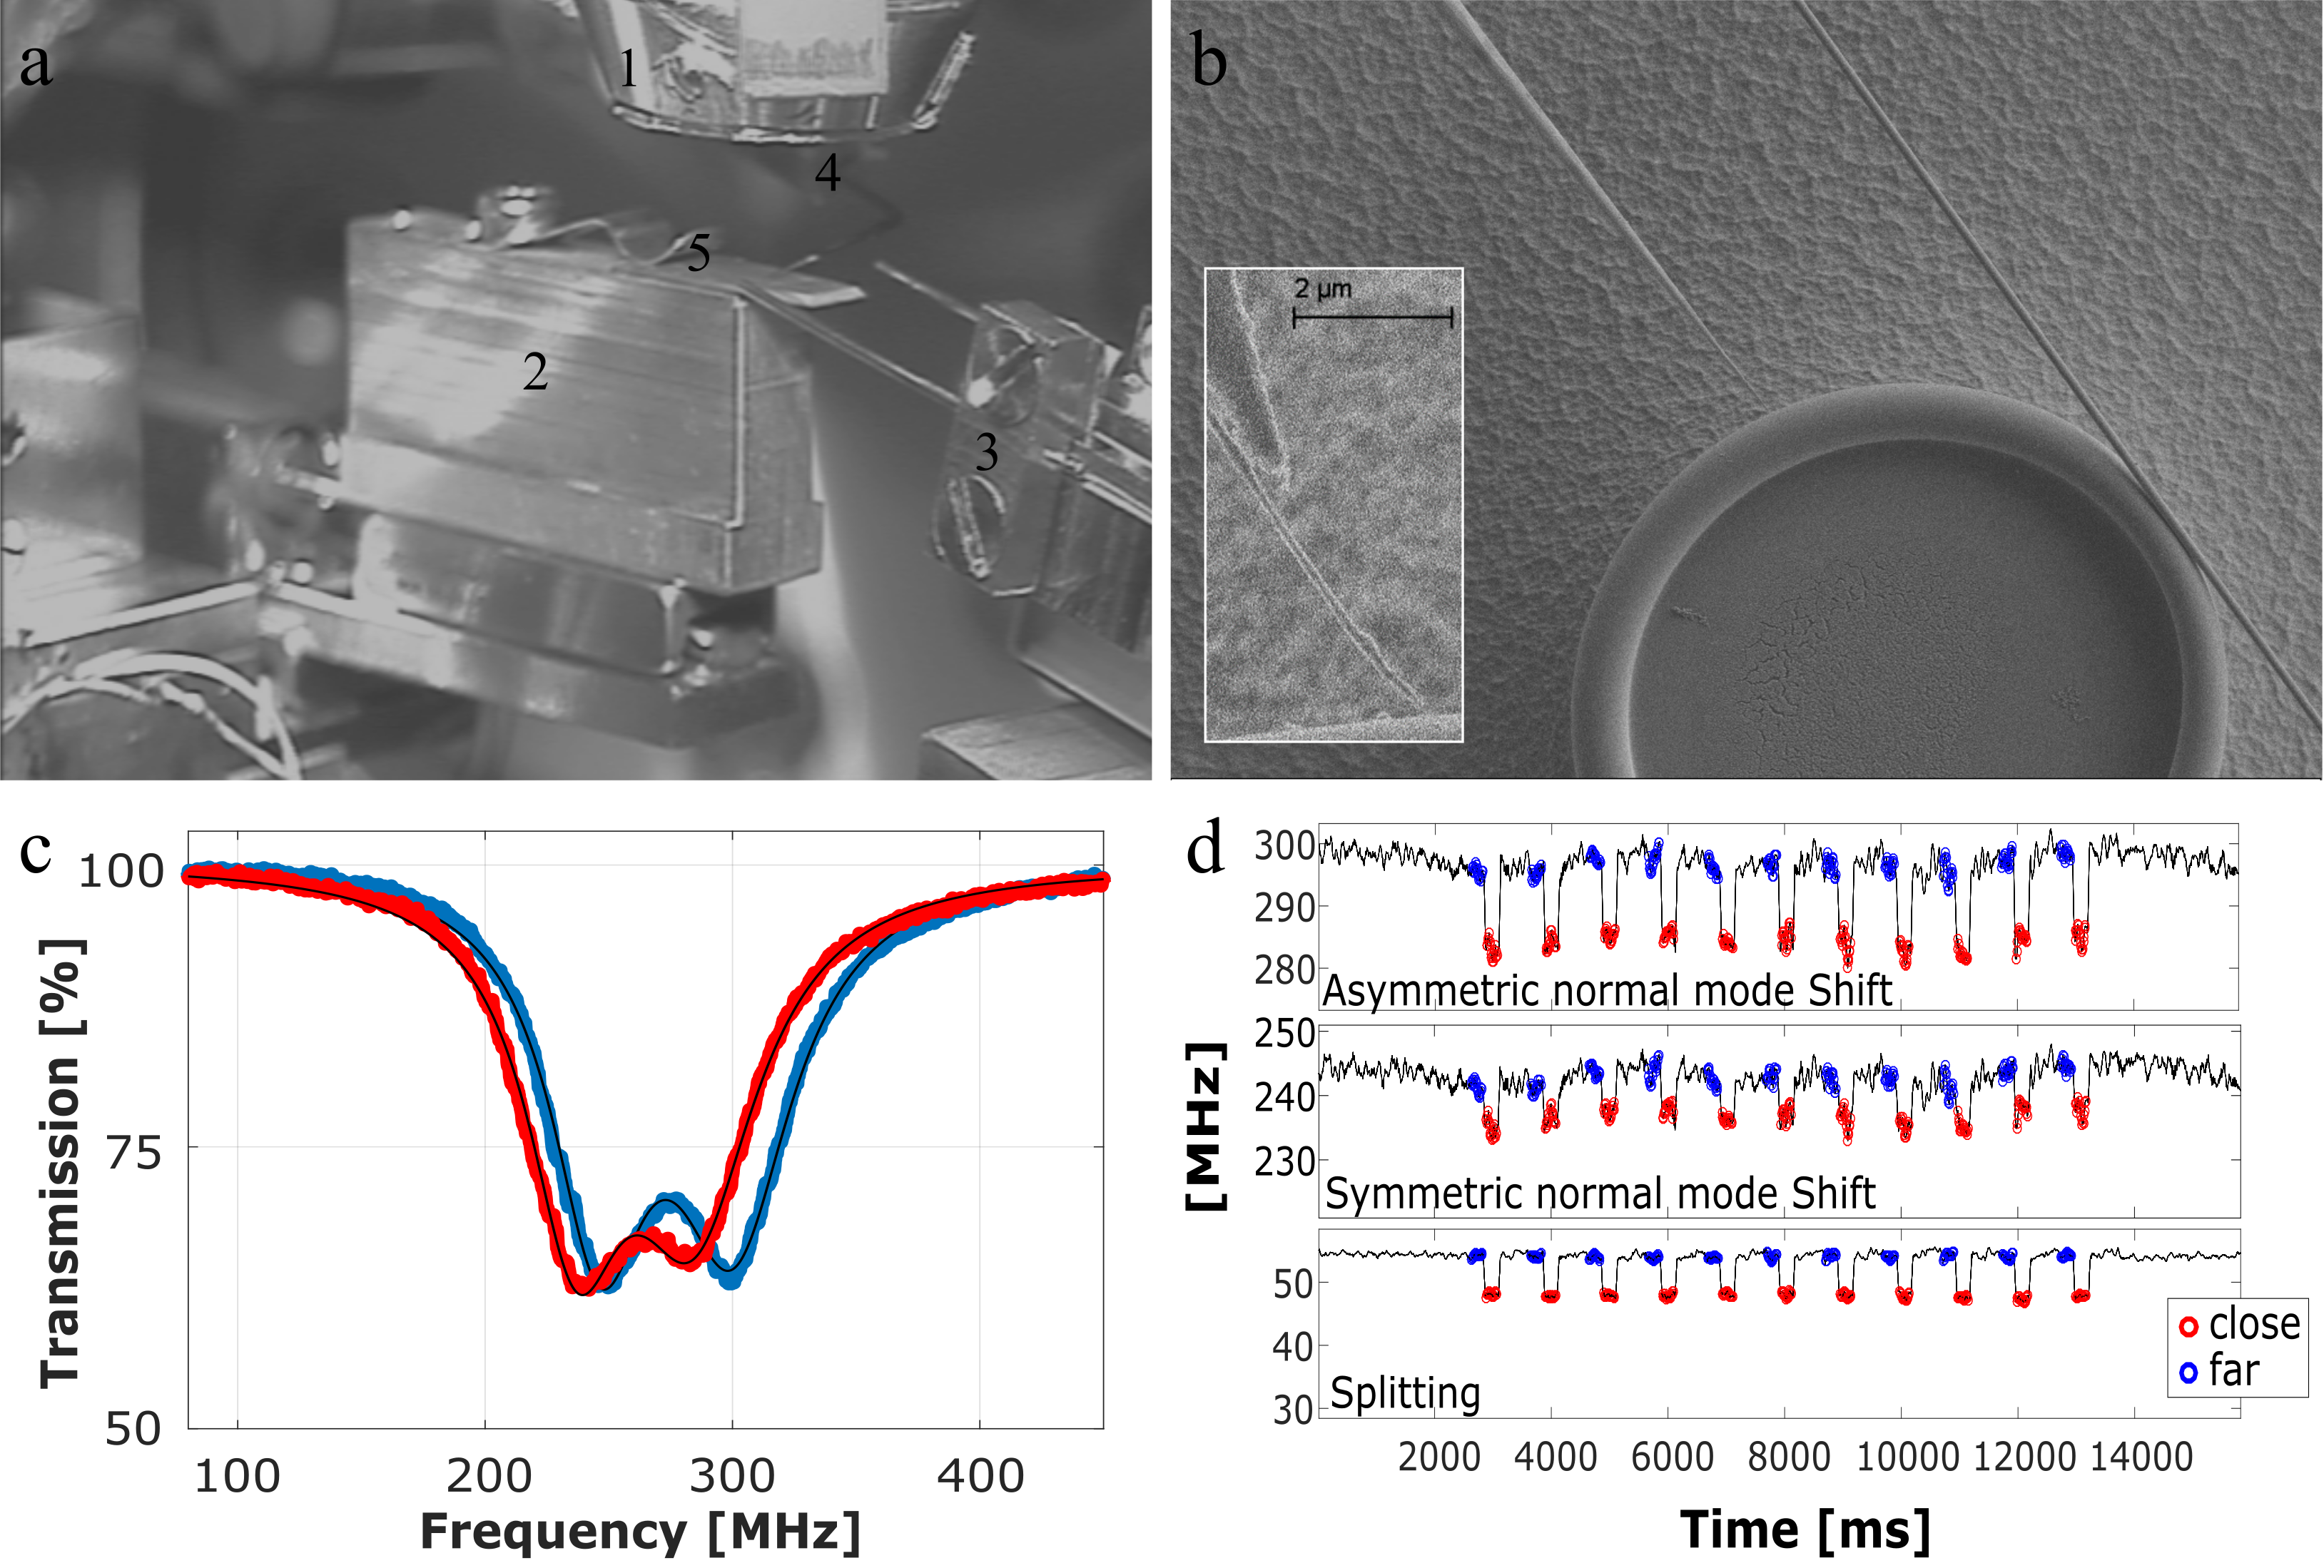
\includegraphics[width=0.95\textwidth]{Images/figure_3_v4.png}
    \caption{\textbf{Measurement of the induced spectral changes.} \textbf{a,} Image of the experimental setup inside the SEM (Zeiss Supra\textsuperscript{TM}). \textbf{1,} SEM objective, \textbf{2,} Resonator chip positioned on a XYZ piezo-actuator Klocke Nanotechnik\textsuperscript{TM} , \textbf{3,} Home-built Nanofiber holder and stretcher mounted on the SEMs positioning system, \textbf{4,} Kleindiek\textsuperscript{TM} nano-manipulator on which the nanotip and nanotube are mounted, \textbf{5,} WGM silicon chip accommodating about 30 resonators. \textbf{b,} The tapered coupled microtoroid with a nanotip brought close to the microresonator surface. \textbf{Inset:} Close-up of the nanotube mounted on the nanotip near the resonators surface. \textbf{c,} A recorded spectra of the microtoroid with the nanotube outside (blue curve) and inside (red curve) the optical mode. The black curves are fits to a Lorentzian doublet. The bare cavity fitted parameters are: $h=29$MHz and $\kappa=28$MHz. \textbf{d,} The recorded center frequencies of the two normal modes and the splitting between them change in time. Top: The asymmetric normal mode center frequency. Center: The symmetric normal mode center frequency. Bottom: The resulting splitting. The blue circles mark the values when the nanotube is out of the mode (far) and the red circles mark the values when the nanotube is positioned inside the evanescent field, as close as possible to the surface without making contact. The induced splitting is twice of $\Delta \omega = 3.4$MHz. The average shift of the center frequency, $\textit S \omega$, is $10$MHz. This gives us a 'normalized induced splitting' of $0.34$, in this example. The presented signals of center frequency were corrected for a linear drift due to thermal effects. The splitting signal is the difference between the raw data of the central frequencies. Note that in this specific position the counter-propagating coupling induced by the nanotube is opposite in sign to the intrinsic coupling $h$, and therefore decreases the overall measured splitting.
		\label{fig:experiment}}
\end{figure}

\section{Results}

\subsection{Induced spectral changes of the TE mode vs. the position along the equator}

In our theoretical model we derive the new eigenfrequencies of the cavity with a non-spherical nanoparticle and arrive to the normalized induced splitting vs. the position along the equator (For full expression see Supplementary Material). for the TE mode in the parametric regime: $h\gg g, \gamma$, we can use the following approximated expression:
\begin{equation}
\frac{\Delta \omega_{TE}}{S\omega}  \approx \frac{1}{g_{k,k}}(\sqrt{ g^2 + 2  g h \cos{2 k x}  + h^2}-h)
\label{eq: delta_omega_approxTE}
\end{equation}
where the average shift is: $\textit{S}\omega=g_{k,k}$.
Note that the approximated expression for $\Delta \omega_{TE} $ (Eq.~\ref{eq: delta_omega_approxTE}) is consistent with previous works~\cite{he2013statistics}, where it was used to describe the interaction of a linearly polarized optical mode, without initial intrinsic splitting, with two isotropic spherical particles

\begin{figure}[H]
\centering
   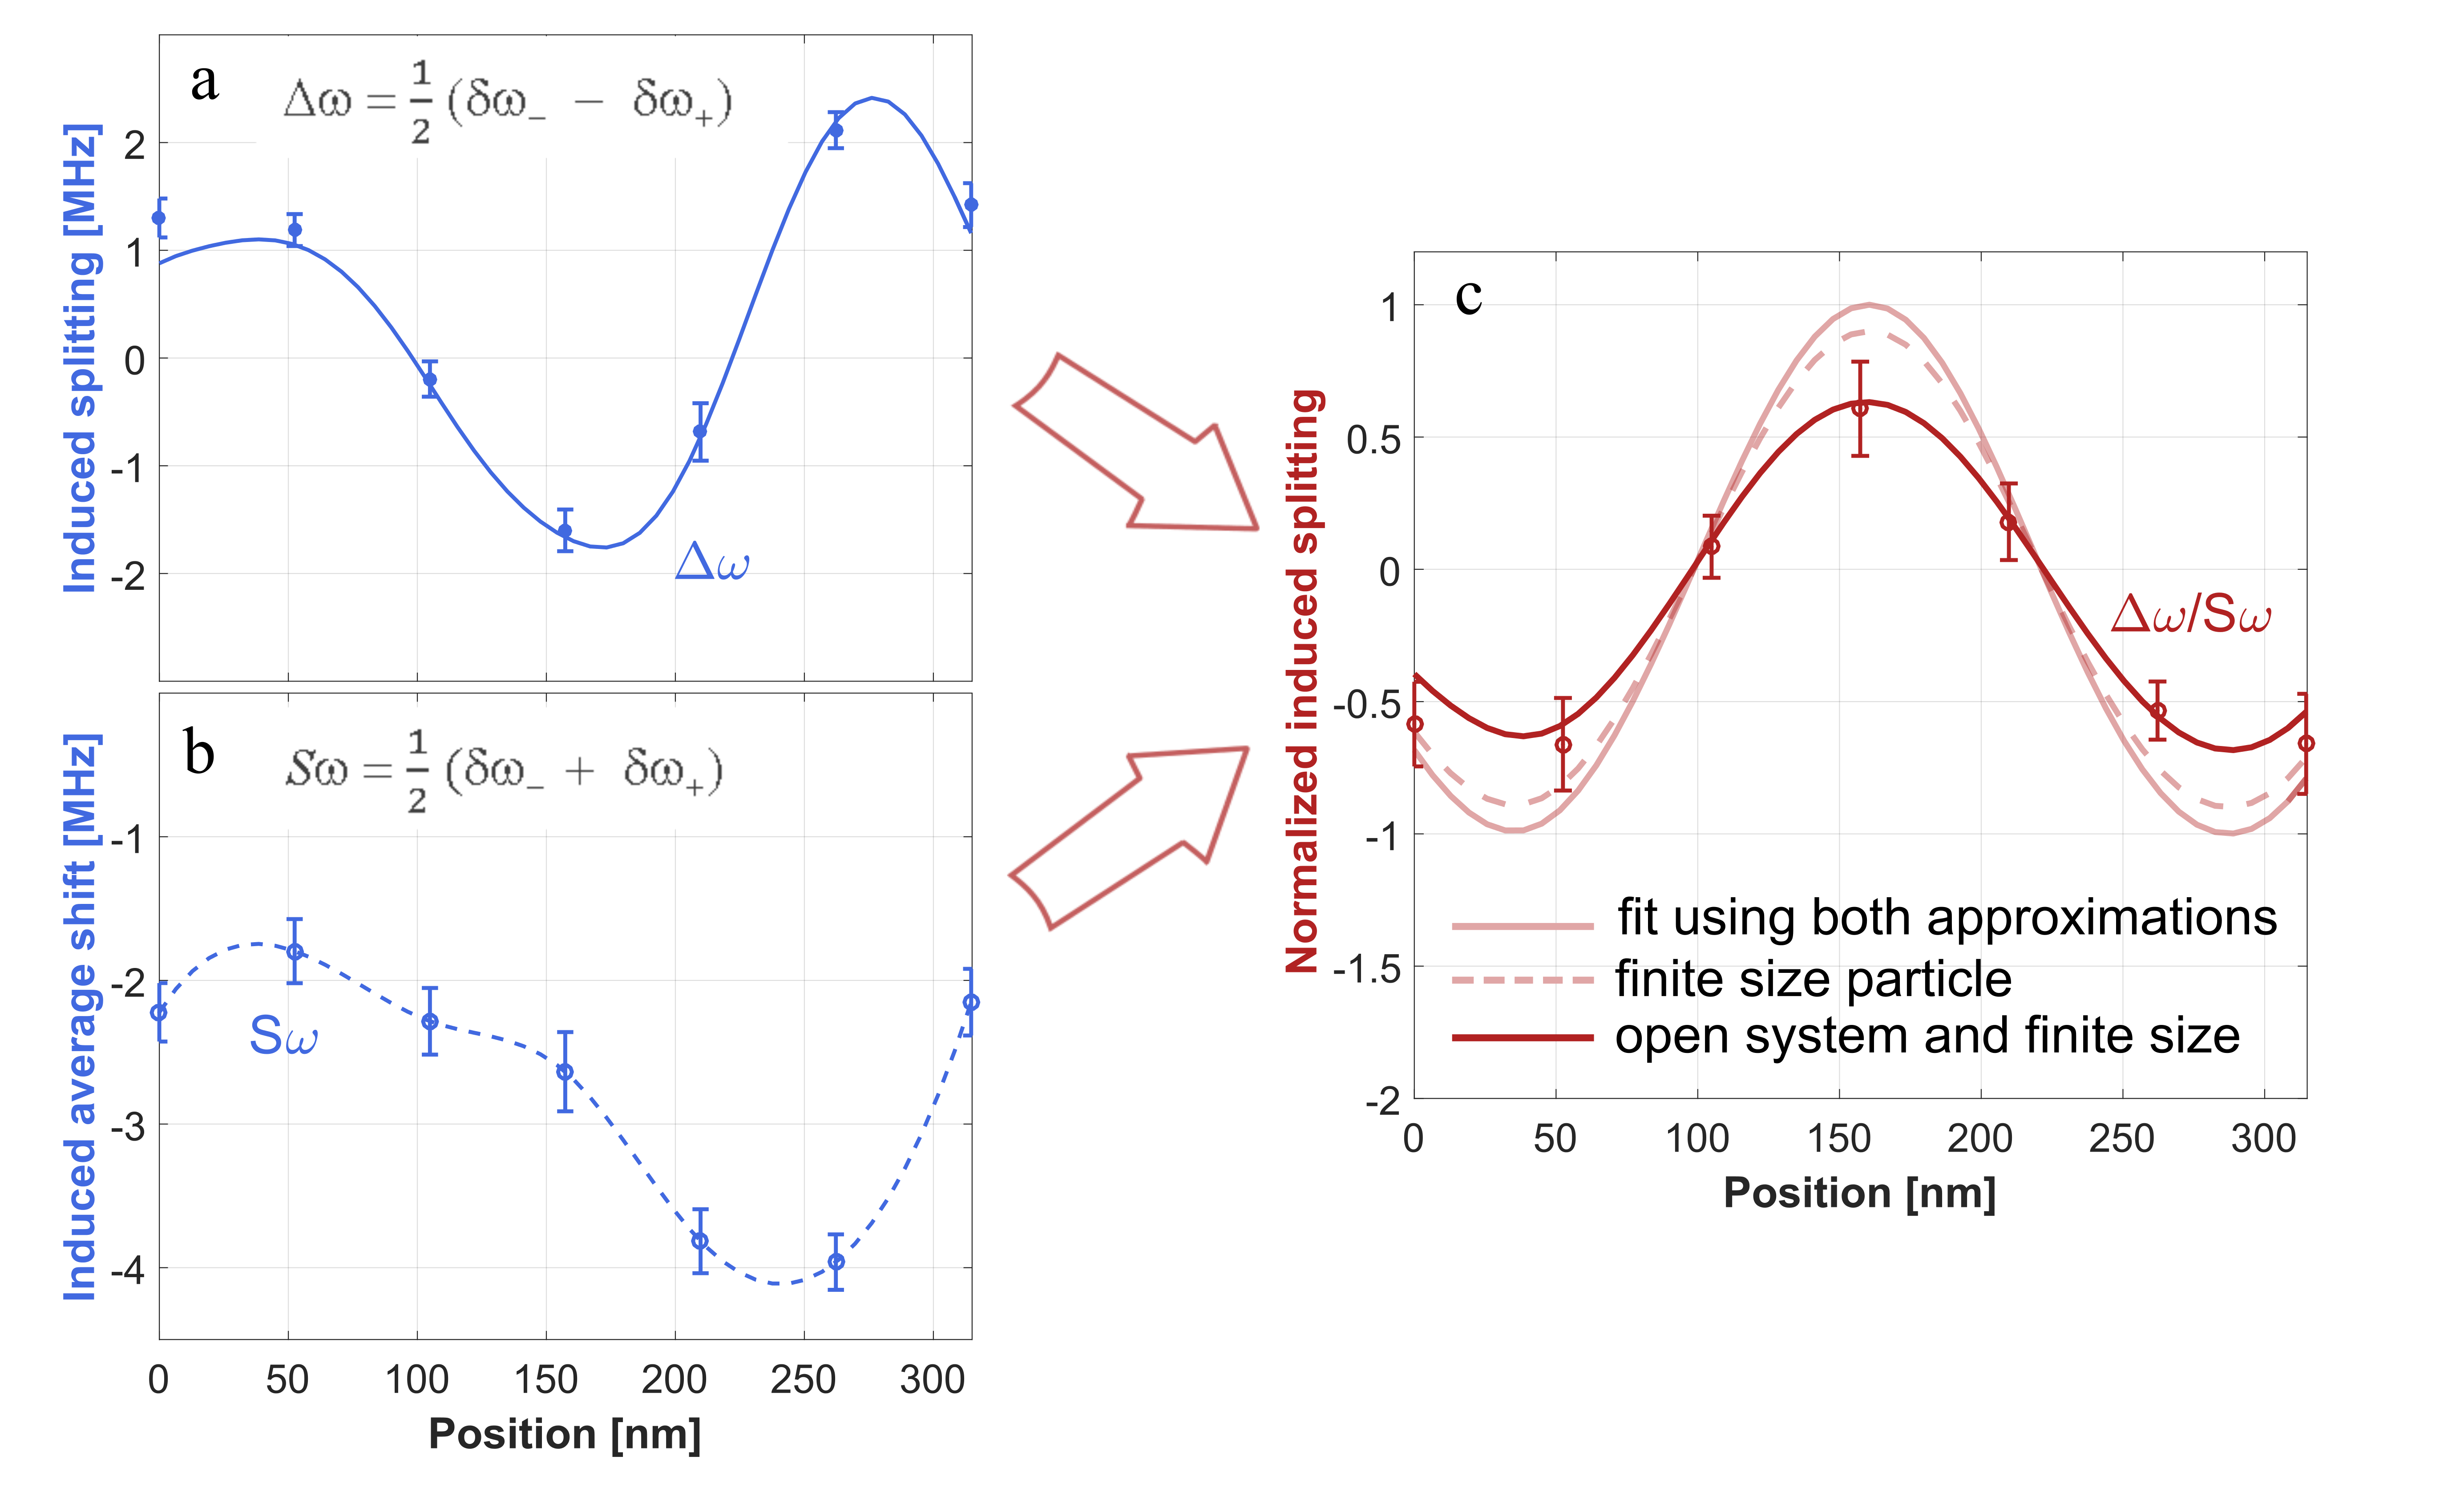
\includegraphics[width=0.95\textwidth]{Images/data_plot_19_TE_forPaper_subplot1C.png}
        \caption{\textbf{Scan results of a TE mode and demonstration of the self-referenced method and open system nature.} (a) The measured half induced splitting between the normal modes of the TE mode vs. the position of the nanotube along the equator. The blue curve is the theoretical prediction of $\Delta \omega$ using the interpolated line (dashed blue line in (c)) from $\textit{S}\omega$ measured data. (b) The measured average shift $\textit{S}\omega$ of the two normal modes in the same measurement. (c) The normalized induced splitting data (the red circles) along with three options for a fit. The light red curve represents the fit to eq.~\ref{eq: delta_omega_approxTE} with the backscattering between the counterpropagating modes being symmetric. This represents the case where the coupling rate between the counterpropagating modes and the coupling rate into the same mode are equal. The light dashed red curve represents an improved fit, where the reference to the size of the particle is included in the model. The dark red solid curve is the best fit to the expression in eq.~\ref{eq: delta_omega_approxTE}, where both the particle size and open system nature is taken into account.}
\label{fig:TE_set19_splitting}
\end{figure}

In the experiment, we scan the nanotube positioning along the equator while it is being held horizontally, perpendicular to the surface of the microtoroid. The spectra are collected with the nanotube inside and outside the optical mode at intervals of 45nm for a total range of at least one wavelength. Then we measure the normalized induced splitting and difference in broadenings vs. the position of the nanotube for the TE and TM modes independently. The measurement with linearly polarized TE mode allows the extraction of the polarizability of the nanotube along a single axis, assuming that the mode properties and the position inside the optical mode are known.

The induced splitting and the induced average shift of the TE normal modes vs. the position along the equator are plotted in Fig.~\ref{fig:TE_set19_splitting}a,b. The blue circle markers represent the measured data: half the splitting ($\Delta \omega$) and the average shift ($\textit{S} \omega$) and the blue curves are guide to the eye (using the non-approximated expression: $\Delta\omega = \frac{1}{2}Re\{\delta\omega_- -\delta\omega_+\}-h$.).

From these results, we can extract the real part of the polarizability along a single axis. In the current configuration the TE field probes the short axis of the nanotube, giving $\mathcal{R}e(\alpha_{\perp})$. To estimate the polarizability we can use the measured average induced shift ($S\omega = (2.7 \pm 0.85$)MHz in the current experiment) or the coupling rate between the counterpropagating modes from fit to the ($\Delta \omega$) data. However, these measurements also depend on the parameters of the optical mode, such as the mode volume and the exact position of the nanotube inside the evanescent field in the radial direction, which are sometimes hard to evaluate. For example, we see (Fig.~\ref{fig:TE_set19_splitting}b) that although the average shift signal $S\omega$ is not supposed to be modulated with the position on the equator, we still observe its variations. The same dependence on the mode properties exists in the induced splitting signal.

To cancel out this position-dependent variation and to overcome the randomness of the nanotube positioning within the standing wave pattern, we propose here a method for a self-referenced measurement that involves normalizing of the induced splitting, $2\Delta\omega$, with the induced total shift, $2S\omega$. This ratio, taken at each measurement point, is plotted in Fig.~\ref{fig:TE_set19_splitting}c along with three types of fits to the data.

The strength of the model is demonstrated by first plotting the fit according to the expression that assumes a closed system approximation and does not take into account the size of the particle relative to the standing wave pattern (light red). This fit has a modulation depth of one, as the coupling rate between the counterpropagating modes and the coupling rate into the same mode are equal. ($g_{k,k}=g$ in eq.~\ref{eq: delta_omega_approxTE}). We see that this curve does not describe the measured data. Second, we plot the fit that takes into account that the diameter of the nanotube is $60nm$ and the periodicity of the standing wave is $\sim 250nm$, for the wavelength of $\sim740nm$ (dash red). This reduces the modulation depth to $0.9$. Lastly, we plot the fit that takes into account both the size of the particle and that the approximation to a closed system does not describe the system accurately and the standing wave pattern has a traveling component (solid dark red). In this case, the modulation depth is only $\sim0.6$. This demonstrates that these aspects, that we introduced into our model, influence drastically (could be by $40\%$) the accuracy of the particle characterization and sizing.

\subsection{Characterization of a uniaxial particle using the TM mode}

We can fully characterize a uniaxial particle (single \ce{WS_2} nanotube) solemnly with the TM mode. The normalized induced splitting and the normalized induced difference in broadening of the two TM normal modes vs. the position on the equator are plotted in Fig.~\ref{fig:TM_width_splitting}.

\begin{figure}[H]
\centering
   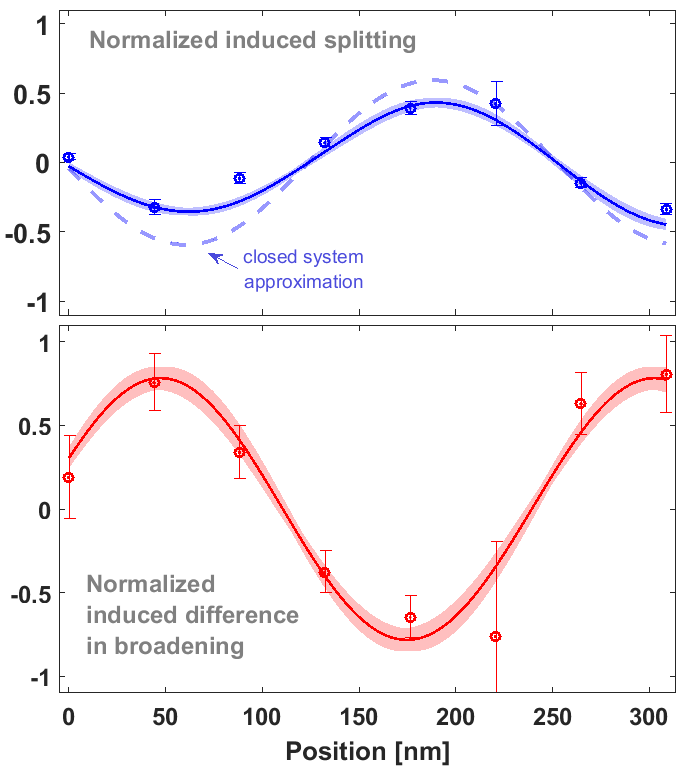
\includegraphics[width=0.5\textwidth]{Images/NTset5TM-addphase038.png}\\
    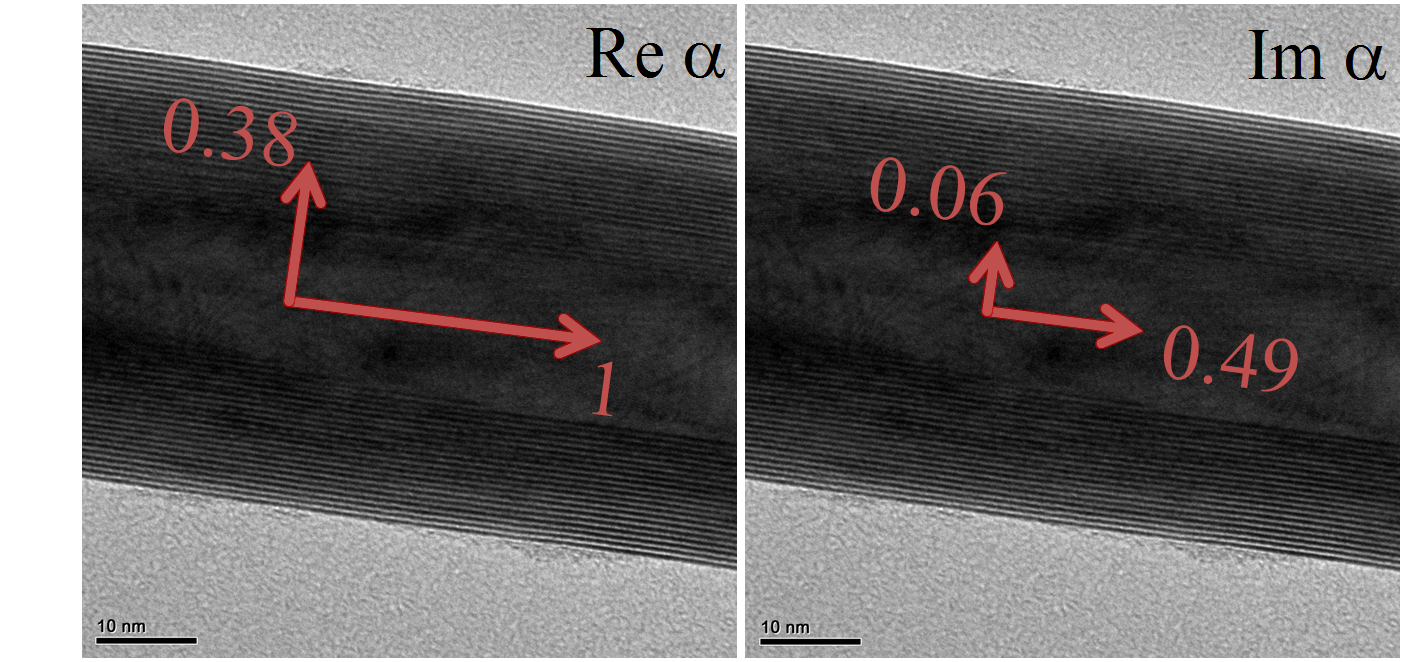
\includegraphics[width=0.475\textwidth]{Images/TEM_NT_ratio_038A.png}
    \caption{ \textbf{a,} The normalized induced splitting (top) and the normalized induced difference in broadening (bottom) between the symmetric and the antisymmetric normal modes of the TM mode vs. the position of the nanotube along the equator. Top: The normalized induced splitting is obtained according to the method described for the TE measurement, (Fig.~\ref{fig:TE_set19_splitting}). The data ($\Delta \omega / \textit{S} \omega$) is marked by the blue circles. The blue curve is the best fit to the data using eq.~\ref{eq:delta_omega_approxTM} and the shaded range indicates the $95\%$ confidence intervals of the fit.
    The dashed blue light curve is the best fit for the normalized induced splitting without the correction for an open system. Bottom: The data ($\Delta \Gamma / \textit{S} \Gamma$) marked with the red circles. The red curve is the best fit to the normalized and the shaded range indicates the $95\%$ confidence intervals of the fit.
    \textbf{b,} Summary of the measured $R_{re}=0.38$, $R_{im}=0.12$, $R_{im/re}^{||}=0.5$ and $R_{im/re}^{\perp}=0.16$ polarizability ratios on top of a TEM (Transmission electron microscope) image of a typical \ce{WS_2} nanotube as  used in our work. The scale-bar of the TEM image of the nanotube is $10nm$.}
\label{fig:TM_width_splitting}
\end{figure}

The induced normalized splitting of the TM mode according to our theoretical model is:
\begin{equation}\label{eq:delta_omega_approxTM}
         \frac{\Delta \omega}{S\omega} = \frac{\sqrt{g^2 + g_{cp}^2 + 2 g h \cos{2 k x} - 2 g_{cp} h \sin{2 k x} + h^2}-h}{g_{k,k}}
\end{equation}
The expression to normalized induced broadening is given in the Supplementary material.
The fitted parameters from the two fits in Fig.~\ref{fig:TM_width_splitting} are:
\begin{equation}\label{eq:fitting_parameters}
  \begin{split}
     \tilde{g} &= 0.65 \pm 0.03 ~~~~~~~~      \tilde g_{cp} = 0.09 \pm 0.01\\
       \tilde {\gamma}&= 0.86 \pm 0.04 ~~~~   \tilde{\gamma}_{cp} = 0.16 \pm 0.02
   \end{split}
\end{equation}
where the $tilde$ sign corresponds to the normalized values of $g$ and $g_{cp}$ by the coupling rate into the same mode, $g_{k,k}$, and of $\gamma$, $\gamma_{cp}$ by the $\gamma_{k,k}$ loss rate. These normalization terms are obtained from the average induced shift and average induced broadening of the resonances by taking the mean of the measurements at all locations:
\begin{equation}\label{eq:dc_parameters}
  \begin{split}
     \textit{S}\omega=g_{k,k} &= 9.9 \pm 3.3 MHz   \\
      \textit{S}\Gamma=\gamma_{k,k} & = 4.3 \pm 1.7 MHz
  \end{split}
\end{equation}
where the error range marks the standard errors of the fits.

\subsection{Extraction of the polarizability ratios}

\textbf{Polarizability ratios definition.} Our goal is to characterize of a non-spherical particle by measuring the polarizability ratios between the different components of the polarizability tensor. The polarizability ratios are often used to characterize non-spherical structures such as carbon nanotubes~\cite{rao2000polarized,reich2000comment,wang2004receiving} or various inorganic nanotubes, such as \ce{WS_2} nanotubes~\cite{tenne2005orientation,yang2008phototransistors} and are defined here as well. The polarizability ratios are defined by:
\begin{equation}\label{ratio_definitions}
\begin{split}
   R_{re}  &= \frac{\alpha^{re}_{\perp}}{\alpha^{re}_{||}}; ~~~~~~~~~
    R_{im}  = \frac{\alpha^{im}_{\perp}}{\alpha^{im}_{||}}; \\
    R_{im/re}^{||}  &= \frac{\alpha^{re}_{||}}{\alpha^{im}_{||}} ~~~~~~~~~
    R_{im/re}^{\perp}  = \frac{\alpha^{re}_{\perp}}{\alpha^{im}_{\perp}}
\end{split}
\end{equation}
Three of these ratios dictate the fourth.

Using the fitted normalized induced splitting (eq.~\ref{eq:delta_omega_approxTM}) and the known orientation of the nanotube we extract $R_{re}$, and similarly $R_{im}$ is extracted from the fit to the normalized difference in broadening.
The ratio between the real and the imaginary parts of the polarizability $R_{im/re}^{||}$
is obtained from the ratio between the average shift to the average broadening: $\frac{\textit{S} \omega} {\textit{S} \Gamma}$ where $\textit{S} \Gamma= \gamma_{t,k,k}=\gamma_{s,k,k}+\gamma_{a,k,k}$. However, in our case  the cross section for scattering is small, hence the ratio becomes simply:
\begin{equation}\label{eq:Rre_im_noscatt}
   \frac{\textit{S} \omega} {\textit{S} \Gamma}=\frac{g_{k,k}}{\gamma_{a,k,k}}\approx \frac{Re ( \alpha_{||} )}{Im (\alpha_{||})} = R_{im/re}^{||}
\end{equation}

\textbf{Measured polarizability ratios.} The measured polarizability ratios for the nanotube are as follows:
\begin{equation}\label{eq:ratios_nanotube}
\begin{split}
  & R_{re}  = 0.38 \pm 0.05 \\
   & R_{im}  = 0.12 \pm 0.06\\
   & R_{im/re}^{||}  = 0.5 \pm 0.05 \\
   &R_{im/re}^{\perp}=0.16 \pm 0.8
\end{split}
\end{equation}
In the following discussion we address in detail each of the polarizability ratios, $R_{re}$, $R_{im}$ and $R_{im/re}^{||}$. We approximate the end of the nanotube that enters the optical mode by a prolate ellipsoid and calculate the polarizability of an ellipsoid~\cite{hulst1957light}. We use the measured diameter of the nanotube $58nm \pm 2nm$. The exact length of the nanotube inside the mode is not well-defined so we make our calculations assuming an ellipsoid with a varying length. The ellipsoid length corresponds to the overlap of the nanotube with the optical mode (overlap length).  The permittivities that are used for the calculations are $\epsilon_{||}=14.26-i0.55$ and $\epsilon_{\perp}=10.3-i0.2$~\cite{taverna2002}.

Fig.~\ref{fig:pol_ratios}a presents the comparison of the measured value for the ratio between the real parts of the polarizability $R_{re}=Re (\alpha_{\perp}) \Big/ Re(\alpha_{||})=0.38 \pm 0.05$, (blue dot) to the calculated value of $R_{re}$ ratio vs. the overlap length(blue curve). The estimated overlap length in our measurement is $130nm$, which is given by our FEM simulation in Comsol (see methods).
The dashed black curve represents the polarizability ratio for bulk \ce{WS_2}:
\begin{equation}\label{eq:Rre_bulk}
R_{re}^{bulk}=\frac{\epsilon_{\perp}'-1}{\epsilon_{||}'-1}=0.48
\end{equation}
The ratio $R_{re}=0.16\pm0.05$ of a single suspended nanotube was measured previously in the far-field regime, using Raman Spectroscopy~\cite{tenne2005orientation} (green dot in Fig.~\ref{fig:pol_ratios}a). In that work an individual multiwalled \ce{WS_2} nanotube with an outer diameter of $15-25nm$ was placed on an AFM tip and illuminated with linearly polarized light ($633nm$) at different angles to the axis of the nanotube. The overlap length corresponds to the spot size of $\sim1um$ that was used.
The green dash-dot curve in Fig.~\ref{fig:pol_ratios}a represents the calculated $R_{re}$ for a nanotube with an outer diameter of $25nm$ at a wavelength of $633$nm.

\begin{figure}[H]
\centering
   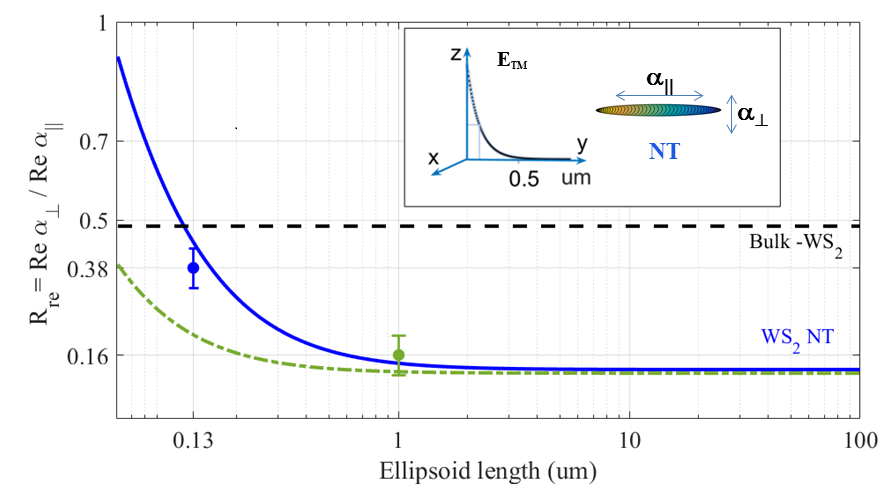
\includegraphics[width=0.475\textwidth]{Images/Rre_semilog_NT91A.png}\\
   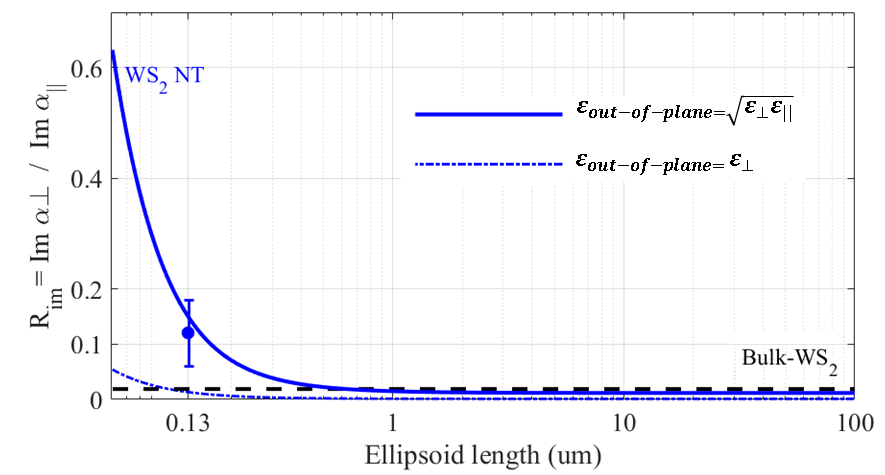
\includegraphics[width=0.475\textwidth]{Images/Rim_semilog_NT6_a1.png}\\
   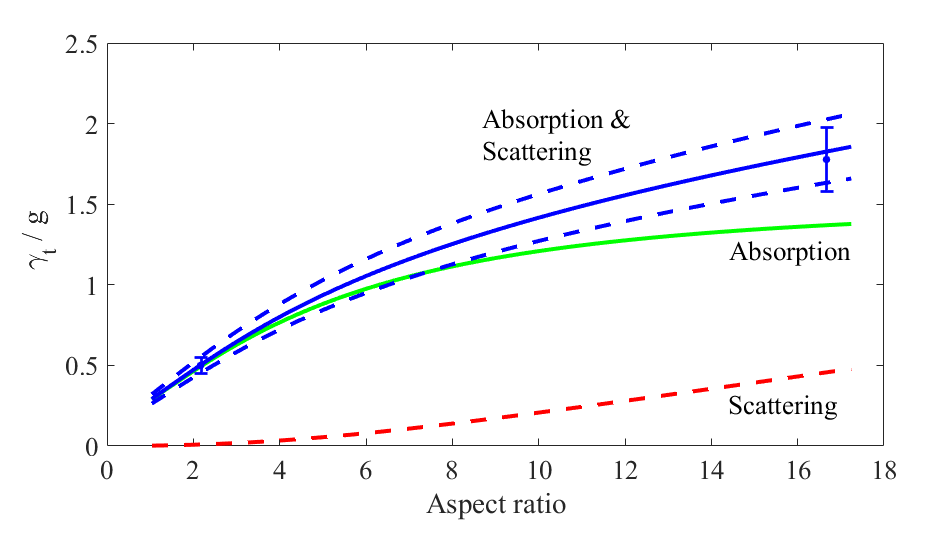
\includegraphics[width=0.475\textwidth]{Images/R_re_im_with_scattering.png}
   \caption{\textbf{The calculated and the measured polarizability ratios of the \ce{WS_2} nanotube.} \textbf{a,} The calculated ratio between the real parts of the polarizabilities $R_{re}$ of a \ce{WS_2} nanotube vs. the overlap length between the nanotube and the optical mode (blue curve) (See Methods). The measured polarizability ratios are shown: The first (blue circle) $0.38 \pm 0.05$ is measured in our experiment and the second (green circle) $0.16.\pm0.05$ was measured previously for a similar type of nanotubes at a wavelength of 633nm~\cite{tenne2005orientation}. The green dash-dot curve is the calculated polarizability ratio for a $25nm$ outer diameter nanotube illuminated with $633nm$ light. The dashed black curve represents the polarizability ratio for bulk-\ce{WS_2}. \textbf{b,} The calculated ratio between the imaginary parts of the polarizabilities $R_{im}$ of a \ce{WS_2} nanotube vs. the overlap length between the nanotube and the optical mode assuming effective permittivity (blue curve) and when taking the normal one (dotted curve). The measured imaginary parts polarizability ratio is shown to be in good agreement with the curve plotted using the corrected effective permittivity (blue circle). \textbf{c,}}
\label{fig:pol_ratios}
\end{figure}

In Fig.~\ref{fig:pol_ratios}b, the measured ratio between the imaginary parts of the polarizability $ R_{im}=Im (\alpha_{\perp}) \Big/ Im(\alpha_{||})=0.12\pm0.06$ is plotted (blue dot) along with the calculated ratio vs. the overlap length (blue solid curve). Note that in all our calculations for the polarizability along the short axis of the nanotube we use an effective value of permittivity: $\sqrt{\epsilon_{\perp}\epsilon_{||}}$~\cite{taverna2002,kociak2001experimental}. The reason is the fact that in the multiwall nanotube of such small radius ($\sim 30nm$) the principal crystallographic axis (defined perpendicular to the \ce{WS_2} sheets) changes rapidly on the scale of the nanostructure, thus both the in-plane and out-of-plane components of the dielectric tensor contribute to the out-of-plane polarizability calculation. The dash-dot blue curve in Fig.~\ref{fig:pol_ratios}b represents the calculated polarizability ratio without this adaptation. We see that indeed using the adapted value leads to a much better agreement. The dashed black curve represents the calculated value for the bulk-\ce{WS_2}:
\begin{equation}\label{eq:Rim_bulk}
  \frac{\epsilon_{\perp}''}{\epsilon_{\parallel}''}=0.017.
\end{equation}

The ratio of the imaginary to real parts of the polarizability $R_{im/re}^{||}$ of the nanotube in horizontal orientation is measured to be $0.5 \pm 0.05$ and $R_{im/re}^{\perp}=0.16 \pm 0.8$ (eq.~\ref{eq:ratios_nanotube}). For a nanotube in vertical orientation: $R_{im/re}^{||}=1.78 \pm 0.18$ and $R_{im/re}^{\perp}=0.6 \pm 0.1$. The calculated ratios for bulk-\ce{WS_2} are:
\begin{equation}\label{eq:Rre_im_bulk}
  R_{im/re,bulk}^{||}=\frac{\epsilon_{||}''}{\epsilon_{||}'-1}=0.04
\end{equation}
\begin{equation}\label{eq:Rre_im_bulk_perp}
    R_{im/re,bulk}^{\perp}=\frac{\epsilon_\perp''}{\epsilon_\perp'-1}=0.0015
\end{equation}
We see that the in-plane ratio ($R_{im/re}^{||}$) for the \ce{WS_2} nanotube is $\sim12$ times larger than the ratio for bulk-\ce{WS_2}. The out-of-plane ratio ($R_{im/re}^{\perp}$) is $\sim106$ times larger than the bulk ratio. We believe this is attributed to the fact that the imaginary part of the permittivity is higher in the nanotube than in bulk, whereas there is a decrease of the real part. Specifically, the direct band-gap of bulk 2H-WS$_2$ is at $2.04$eV ($\lambda=608nm$)~\cite{wilson1969transition}, the indirect band-gap at $1.3$eV ($\lambda=954nm$)~\cite{ballif1999optical} and exciton A is at $1.95$eV ($\lambda=636nm$)~\cite{frey1998optical}. The optical absorption of nanotubes was believed to have the same features~\cite{frey1998optical} as the bulk. However, recent work~\cite{Yadgarov2016unique} proves the presence of both excitonic and plasmonic features. Namely, the nanotubes preserve their \ce{WS_2} bulk properties but also maintain a plasmonic resonance at $\sim 600nm$. Our illumination, at $735nm$, is detuned from all these transitions and the plasmonic resonance. Hence, we can assume that we measure the plasmonic off-resonance response, being red-detuned by $\sim135nm$ from the plasmon resonance center.
Different loss mechanism contributes to the imaginary part of the dielectric function, and one of them might be oscillations of the free charge, a plasmon~\cite{Yadgarov2016unique}. This could explain the increased by an order of a magnitude imaginary part of the permittivity.

Another supporting recent work is by Levi at al.~\cite{levi2013}, which measured the conductivity of a single $\ce{WS_2}$ nanotube using a nanotube-based transistor and find it to be six orders higher than in similar dichalcogenide multilayer-devices. Even though this comparison of the conductivity with other works does not differentiate between better or worse performed ohmic contacts and changes in the measurement environment, such as air or vacuum, an unexpectedly high charge density was measured for a \ce{WS_2} nanotube relatively to 2H-\ce{WS_2} bulk.

\section{Discussion}

In this work, we present a model for light-matter interactions of arbitrarily shaped nano-object with linear (TE) or elliptical (TM) polarization optical modes. We then implement a measurement scheme that allows $3D$ characterization and measurement of the polarizability ratios of arbitrarily shaped nano-object using a WGM microresonator. In particular, the spectral changes of the two normal modes of the TM mode induced by a presence of a \ce{WS_2} nanotube are correlated to its polarizability tensor and the polarizability ratios between the real parts, the imaginary parts and the imaginary to real parts of a single \ce{WS_2}  nanotube are measured. The measured polarizability ratios of the \ce{WS_2} nanotube are in accordance with the reported value~\cite{tenne2005orientation} and our estimation form the measured bulk properties.

The presented model introduces important aspects that were often not taken into account such as the implementation for sensing with an open system configuration which is typical in the WGM sensing configurations. When the cavity losses ($\kappa$) are comparable to the coupling rate between the counterpropagating modes ($\textit{h}$) the spectrum has the shape of a not fully resolved doublet and the average steady-state amplitudes of the different modes are not equal in-contrary to the closed system approximation.

In our model, we took this effect into account by applying an iterative calculation. As a first step we assumed to have a closed system ($g_{k,k'}^{(1)} = g_{k,k}$) an extracted the coupling rate by fitting. From this result we calculated the ratio between the amplitudes of the counterpropagating fields ($f$), plugin it back into the coupling rate $g_{k,k}^{(2)} = fg_{k,k}$ and preformed the fit again. This was repeated until the two values converged, $g_{k,k}^{(n+1)} = g_{k,k}^{(n)}$.

To support the proposed method we use the measurement of the nanotube with the TE mode. We show there could be tens of percents of deviation of the estimated coupling rate (and hence the polarizability) when the values are derived under the closed system approximation, and that the full model we propose corrects these deviations.

Additionally, we demonstrate a complementary approach of a self-referenced measurement, which involves a normalization of the splitting or difference in broadening of the two normal modes by the average shift or average broadening of the two normal modes, respectively. In previous works \textbf{[add ref]}, where non-absorbing particle was used, the particle position and mode volume dependence, which are parameters that are hard to accurately predict, were eliminated by dividing the shift with the broadening signal $\delta \omega / \delta \Gamma$. Similarly to the $\delta \omega / \delta \Gamma$ method, the current $\delta \omega / \textit{S} \omega$ normalization technique also eliminates these dependencies. The importance of our method is in a system where the detected particle perturbs the standing wave pattern of the WGM microresonator or in a multiple particle detection that induces splitting. This is because the $\delta \omega / \textit{S} \omega$ measurement tells us where along the standing wave the particle landed. For example, in a measurement of a small nanoparticle of arbitrarily shape that perturbs a well resolved TE mode, $\delta \omega / \textit{S} \omega$ equals one, which tells us that the particle is positioned at a node of the symmetric standing wave pattern. This enables more accurate and less position-dependant, real-time sizing of the particle.

The influence of the nanoparticle size compared to the standing wave pattern was also taken into consideration. This was evaluated by treating the nanoparticle contribution as the integral contributions over infinitesimally small particles along the size of the particle, which effectively can be seen as the convolution of the nanoparticle with the standing wave. For $60nm$ radius particle in a $740 nm$ wavelength, as for this work, we estimate the effect to be $\approx 9\% $ on the modulation depth.
In our work, we did not consider the influence of the evanescent field gradient over the nanoparticle as was presented in the recent work~\cite{foreman2017Whispering}. From this additional effect, we estimated to have an additional $6 \% $ decrease in the modulation depth that is still in corresponds with our experimental results.

We believe that this work sets the grounds for three-dimensional label free sensing of arbitrarily shaped nanoparticles and could be implemented in various detection schemes. Such TE-TM measurements can be harnessed for structural characterization of nano-objects and the detailed measurement of various properties, such as chirality and conformational changes.

%%%%%%%%%%%%%%%%%%%%%%%%%%%%%%%%%%%%%%%%%%%%%%%%%%%%%%%%%%%%%%%%%%%%%
%% The "Acknowledgement" section can be given in all manuscript
%% classes.  This should be given within the "acknowledgement"
%% environment, which will make the correct section or running title.
%%%%%%%%%%%%%%%%%%%%%%%%%%%%%%%%%%%%%%%%%%%%%%%%%%%%%%%%%%%%%%%%%%%%%
\begin{acknowledgement}



\end{acknowledgement}

%%%%%%%%%%%%%%%%%%%%%%%%%%%%%%%%%%%%%%%%%%%%%%%%%%%%%%%%%%%%%%%%%%%%%
%% The same is true for Supporting Information, which should use the
%% suppinfo environment.
%%%%%%%%%%%%%%%%%%%%%%%%%%%%%%%%%%%%%%%%%%%%%%%%%%%%%%%%%%%%%%%%%%%%%
\begin{suppinfo}

We choose the fundamental modes of a Silica microtoroidal cavity at the wavelength of $\sim740nm$ and characterize their polarization (TE or TM) using a side view CCD camera.
The spectrum measurement is performed with a fiber-coupled microtoroid that is placed inside a scanning electron microscope (SEM) chamber that was modified to have an optical fiber feedthrough. A $\ce{WS_2}$ nanotube is brought close to the surface of the microtoroid and placed at the equatorial level, perpendicularly to the surface.

The position of the nanotube near the surface is modulated by approximately $200nm$ peak-to-peak, enough to bring the nanotube in and out of the mode. The spectrum is recorded with the rate of $100$Hz, which is the frequency scan rate of the laser, at $1$MS/sec, which is the maximum sampling rate of our PCI card.

Figure~\ref{fig:pol_ratios} the calculations of the polarizability ratios of the nanotube assume the following permittivities along its two axes: $\epsilon_{||}=14.26-i0.55$ and $\epsilon_{\perp}=10.3-i0.2$~\cite{taverna2002,kociak2001experimental} for the wavelength of $735nm$ and an ellipsoidal particle~\cite{hulst1957light}. The calculation of the polarizabilities of bulk-\ce{WS_2} assume $\epsilon_{||}=14.26-i0.55$ and $\epsilon_{\perp}=7.44-i0.0095$~\cite{taverna2002}.

Comsol simulations: The decay length of the TM field in the microtoroid that was used (major diameter $52um$, minor diameter $8um$) is $120nm$  (see inset in Fig.~\ref{fig:pol_ratios}a) and together with the orientation of the nanotube we get approximately $130nm$ of overlap.

\end{suppinfo}

%%%%%%%%%%%%%%%%%%%%%%%%%%%%%%%%%%%%%%%%%%%%%%%%%%%%%%%%%%%%%%%%%%%%%
%% The appropriate \bibliography command should be placed here.
%% Notice that the class file automatically sets \bibliographystyle
%% and also names the section correctly.
%%%%%%%%%%%%%%%%%%%%%%%%%%%%%%%%%%%%%%%%%%%%%%%%%%%%%%%%%%%%%%%%%%%%%
\bibliography{paper_bib}

\end{document}